\documentclass[11pt]{book}
\usepackage[utf8]{inputenc}
\usepackage{geometry}
\usepackage{tikz}
\usepackage{hyperref}
\usepackage{amsmath}
\usepackage{graphicx}
\usepackage{xwatermark}
\usepackage{eso-pic}
\usepackage{transparent}
\geometry{margin=1in}

% Add watermark on every page
\AddToShipoutPictureBG{%
  
\begin{tikzpicture}[remember picture,overlay]
    % Diagonal watermark pattern
    \foreach \x in {0,2,4,6,8,10,12,14,16,18,20,22,24,26,28,30}
      \foreach \y in {0,2,4,6,8,10,12,14,16,18,20,22,24,26,28,30} {
        \node[rotate=45,text=gray!15,font=\small] at (\x cm,\y cm) {Namelos.xyz};
      }
    % Large centered watermark
    \node[rotate=45,text=gray!08,font=\Huge,anchor=center] at (current page.center) {Namelos.xyz};
    % Corner watermarks
    \node[text=gray!20,font=\tiny,anchor=north west] at (current page.north west) {Namelos.xyz};
    \node[text=gray!20,font=\tiny,anchor=north east] at (current page.north east) {Namelos.xyz};
    \node[text=gray!20,font=\tiny,anchor=south west] at (current page.south west) {Namelos.xyz};
    \node[text=gray!20,font=\tiny,anchor=south east] at (current page.south east) {Namelos.xyz};
  \end{tikzpicture}%
}

\title{Smart Relay: From Networking Basics to AI-Orchestrated VPNs}
\author{tian.shao@namelos.xyz}
\date{\today}

\begin{document}
\maketitle
\tableofcontents

\chapter{Networking Basics}

This chapter builds intuition about how data moves across networks. Understanding these fundamentals is essential for debugging connection issues, designing VPN systems, and interpreting diagnostic information.

\section{OSI Layers in a Nutshell}

The OSI (Open Systems Interconnection) model divides network communication into seven layers. We primarily interact with layers 3--7 when building VPN/proxy systems. The control plane lives in L7, while data plane packets live in L3/L4 tunnels.

\begin{enumerate}
    \item \textbf{Physical Layer (Layer 1)}: Electrical signals, cables, wireless transmission.
    \item \textbf{Data Link Layer (Layer 2)}: Ethernet frames, MAC addresses, local network protocols.
    \item \textbf{Network Layer (Layer 3)}: IP addresses, routing, IP packets.
    \item \textbf{Transport Layer (Layer 4)}: TCP/UDP, ports, reliability, flow control.
    \item \textbf{Session Layer (Layer 5)}: Session management, synchronization.
    \item \textbf{Presentation Layer (Layer 6)}: Data translation, encryption, compression.
    \item \textbf{Application Layer (Layer 7)}: HTTP, HTTPS, DNS, FTP, application protocols.
\end{enumerate}

\section{Simple Path Diagram}
\begin{figure}[h]
    \centering
    
\begin{tikzpicture}[node distance=2cm,>=stealth,thick]
        \node (client) [draw, rounded corners] {Client};
        \node (router) [draw, rounded corners, right of=client] {Router};
        \node (isp) [draw, rounded corners, right of=router] {ISP};
        \node (edge) [draw, rounded corners, right of=isp] {Smart Relay Edge};
        \node (service) [draw, rounded corners, right of=edge] {Service};
        \draw[->] (client) -- node[above]{Ethernet/Wi-Fi} (router);
        \draw[->] (router) -- node[above]{IP} (isp);
        \draw[->] (isp) -- node[above]{Encrypted tunnel} (edge);
        \draw[->] (edge) -- node[above]{HTTP/QUIC} (service);
    \end{tikzpicture}
    \caption{Typical path from client to service via Smart Relay.}
\end{figure}

\section{Key Terms}
\begin{itemize}
    \item \textbf{Latency}: time for a packet to reach the destination.
    \item \textbf{Throughput}: amount of data moved per unit time.
    \item \textbf{Jitter}: variation in latency; hurts real-time traffic.
    \item \textbf{MTU}: maximum packet size before fragmentation.
\end{itemize}

\section{Addresses and Ports Refresher}
\begin{itemize}
    \item IPv4 vs IPv6: plan for dual-stack; IPv6 often less congested.
    \item NAT traversal matters: STUN/TURN not typical for VPN, but port selection affects reachability.
    \item Service differentiation: use ports that blend in (443/8443) but avoid obvious fingerprints.
\end{itemize}

\section{Packet Journey: From Application to Wire}

Understanding how data flows through the network stack helps diagnose issues:

\begin{enumerate}
    \item \textbf{Application Layer}: Your application (browser, VPN client) creates data.
    \item \textbf{Transport Layer}: Data is segmented, port numbers added, TCP/UDP headers created.
    \item \textbf{Network Layer}: IP addresses added, routing decisions made, IP headers created.
    \item \textbf{Data Link Layer}: MAC addresses added, Ethernet frames created.
    \item \textbf{Physical Layer}: Electrical signals sent over cable or wireless.
\end{enumerate}

At each layer, headers are added (encapsulation). When received, headers are removed (decapsulation).

\section{Understanding Connection Failures}

Connection failures can occur at different layers:

\begin{itemize}
    \item \textbf{DNS Failure (Layer 7)}: Cannot resolve hostname to IP address.
    \begin{itemize}
        \item Symptom: "Name or service not known"
        \item Cause: DNS server unreachable, incorrect hostname, DNS misconfiguration.
    \end{itemize}
    
    \item \textbf{Network Unreachable (Layer 3)}: No route to destination.
    \begin{itemize}
        \item Symptom: "Network unreachable", "No route to host"
        \item Cause: Routing table has no entry, firewall blocking, network misconfiguration.
    \end{itemize}
    
    \item \textbf{Connection Refused (Layer 4)}: Port is closed.
    \begin{itemize}
        \item Symptom: "Connection refused", "Connection actively refused"
        \item Cause: Service not running, firewall blocking port, wrong port number.
    \end{itemize}
    
    \item \textbf{Connection Timeout (Layer 4)}: No response to connection attempt.
    \begin{itemize}
        \item Symptom: "Connection timeout", "Operation timed out"
        \item Cause: Firewall silently dropping packets, network congestion, server down.
    \end{itemize}
\end{itemize}

\section{Routing and Packet Forwarding}

When you send a packet, the network stack must decide where to send it:

\begin{enumerate}
    \item Check if destination is on local network (same subnet).
    \item If local, send directly using MAC address (ARP).
    \item If remote, send to default gateway (router).
    \item Router consults routing table to forward packet.
    \item Process repeats at each hop until destination reached.
\end{enumerate}

\textbf{Routing Table Example:}
\begin{verbatim}
Destination     Gateway         Interface
0.0.0.0         192.168.1.1    eth0        # Default route
192.168.1.0     0.0.0.0        eth0        # Local network
10.0.0.0        10.0.0.1       tun0        # VPN network
\end{verbatim}

\section{Firewalls and Packet Filtering}

Firewalls filter packets at different layers:

\begin{itemize}
    \item \textbf{Packet Filtering (Layer 3-4)}: Filter based on IP addresses and ports.
    \item \textbf{Stateful Inspection (Layer 4)}: Track connection state, allow established connections.
    \item \textbf{Application Layer (Layer 7)}: Deep packet inspection, protocol-aware filtering.
\end{itemize}

\textbf{Firewall Behaviors:}
\begin{itemize}
    \item \textbf{Reject}: Send RST packet (connection refused).
    \item \textbf{Drop}: Silently discard packet (connection timeout).
    \item \textbf{Accept}: Allow packet through.
\end{itemize}

Understanding firewall behavior helps interpret connection test results.

\section{Proxy Testing and Troubleshooting}

When testing proxy endpoints, understanding the connection flow helps diagnose issues systematically. This section documents real-world troubleshooting techniques used in Smart Relay.

\subsection{Proxy Connection Flow}

A typical proxy test involves multiple layers:

\begin{enumerate}
    \item \textbf{Local Proxy Startup}: The proxy client (Xray) must start and bind to local ports (SOCKS5, HTTP).
    \item \textbf{Port Readiness Check}: Verify the local proxy ports are actually listening before attempting connections.
    \item \textbf{Outbound Connection}: The proxy client attempts to connect to the remote proxy server (VMess/Shadowsocks endpoint).
    \item \textbf{Test Request}: An HTTP/HTTPS request is made through the local proxy to verify end-to-end connectivity.
\end{enumerate}

\subsection{Common Proxy Testing Issues}

\subsubsection{Issue: "Proxy Server Unreachable"}

\textbf{Symptom}: When testing through SOCKS5 proxy, you get "socks connect error: Proxy server unreachable".

\textbf{Diagnosis Steps}:
\begin{enumerate}
    \item \textbf{Check if proxy process started}: Verify Xray process is running (PID check).
    \item \textbf{Verify port is listening}: Attempt TCP connection to localhost:port (e.g., 127.0.0.1:1080 for SOCKS5).
    \item \textbf{Timing issue}: The proxy may need time to initialize. Wait with exponential backoff (200ms, 400ms, 600ms, etc.).
    \item \textbf{Port conflict}: Another application may be using the port. Check with \texttt{netstat} or \texttt{ss}.
\end{enumerate}

\textbf{Solution}: Implement port readiness checks before testing. In Smart Relay, we check if the SOCKS port accepts TCP connections before attempting HTTP requests through it.

\textbf{Code Pattern}:
\begin{verbatim}
// Wait for proxy to be ready
for attempt in 0..10 {
    sleep(200ms * (attempt + 1));
    if port_is_listening("127.0.0.1", socks_port) {
        break; // Proxy is ready
    }
}
\end{verbatim}

\subsubsection{Issue: "Path / was not found" (404 JSON Errors)}

\textbf{Symptom}: HTTP proxy returns JSON error: \texttt{\{"code":404,"message":"path / was not found"\}}.

\textbf{Root Cause}: When the remote proxy server (VMess/Shadowsocks endpoint) is unreachable, Xray's HTTP proxy cannot forward requests. Instead of returning a proper HTTP error, it may return JSON error responses.

\textbf{Diagnosis}:
\begin{itemize}
    \item The local proxy (Xray) is working (accepting connections).
    \item The outbound connection to the remote server fails.
    \item Xray returns error responses instead of forwarding HTTP requests.
\end{itemize}

\textbf{Solution}: 
\begin{enumerate}
    \item Use SOCKS5 proxy instead of HTTP proxy for testing (more reliable).
    \item Detect JSON error responses and provide clear error messages.
    \item Test multiple endpoints to distinguish local vs remote issues.
\end{enumerate}

\subsubsection{Issue: Connection Timeout to Remote Server}

\textbf{Symptom}: Local proxy works, but connections to remote proxy server timeout.

\textbf{Diagnosis Steps}:
\begin{enumerate}
    \item \textbf{DNS Resolution}: Can you resolve the hostname? Use \texttt{nslookup} or \texttt{dig}.
    \item \textbf{Direct TCP Test}: Try connecting directly to the remote server's IP:port (bypassing proxy).
    \item \textbf{Routing Check}: Use \texttt{traceroute} or \texttt{ping} to see where packets are dropped.
    \item \textbf{Firewall Check}: The remote server's firewall may be blocking your IP or the port.
\end{enumerate}

\textbf{Common Causes}:
\begin{itemize}
    \item Remote server is down or overloaded.
    \item Firewall blocking connections (silent drop = timeout, RST = connection refused).
    \item Network routing issues (packets not reaching destination).
    \item Geographic restrictions (server blocks certain regions).
    \item Protocol mismatch (server requires specific handshake, not plain TCP).
\end{itemize}

\subsection{Best Practices for Proxy Testing}

\subsubsection{Use SOCKS5 for Testing}

SOCKS5 proxy is more reliable than HTTP proxy for connectivity testing:
\begin{itemize}
    \item SOCKS5 operates at a lower layer (Layer 5), closer to TCP.
    \item Less prone to HTTP-specific error handling issues.
    \item Better error reporting when outbound connections fail.
    \item Standard practice in proxy clients (v2rayN, Clash, etc.).
\end{itemize}

\subsubsection{Test URL Selection}

Use reliable, well-known test endpoints:
\begin{itemize}
    \item \texttt{https://www.google.com/generate_204} - Google's connectivity check (returns 204 No Content).
    \item \texttt{https://www.gstatic.com/generate_204} - Google static resources (backup).
    \item \texttt{https://www.apple.com/library/test/success.html} - Apple test page.
    \item \texttt{http://www.msftconnecttest.com/connecttest.txt} - Microsoft connectivity test.
\end{itemize}

These endpoints are:
\begin{itemize}
    \item Highly available (rarely down).
    \item Return predictable status codes (204, 200).
    \item Support both HTTP and HTTPS.
    \item Used by major proxy clients for compatibility.
\end{itemize}

\subsubsection{Port Readiness Verification}

Always verify the proxy port is listening before testing:

\begin{verbatim}
// Pseudo-code for port check
async fn check_port_listening(host: &str, port: u16) -> bool {
    match timeout(1s, TcpStream::connect((host, port))).await {
        Ok(Ok(_)) => true,  // Port is listening
        _ => false,         // Port not ready or unreachable
    }
}
\end{verbatim}

\subsubsection{Error Message Clarity}

Provide clear, actionable error messages:
\begin{itemize}
    \item Distinguish between local proxy issues vs remote server issues.
    \item Include the endpoint address (host:port) in error messages.
    \item Explain what the error means (e.g., "Remote proxy unreachable" vs "Local proxy not ready").
    \item Suggest next steps (check firewall, verify endpoint, etc.).
\end{itemize}

\subsection{Network Diagnostic Tools}

When troubleshooting proxy issues, use these tools:

\begin{itemize}
    \item \textbf{netstat / ss}: Check if ports are listening.
    \begin{verbatim}
    netstat -an | findstr :1080    # Windows
    ss -tlnp | grep :1080          # Linux
    \end{verbatim}
    
    \item \textbf{telnet / nc}: Test TCP connectivity.
    \begin{verbatim}
    telnet 127.0.0.1 1080          # Test local proxy
    nc -zv remote-host 443         # Test remote server
    \end{verbatim}
    
    \item \textbf{curl}: Test HTTP through proxy.
    \begin{verbatim}
    curl -x socks5://127.0.0.1:1080 https://www.google.com
    \end{verbatim}
    
    \item \textbf{traceroute / tracert}: Check routing path.
    \begin{verbatim}
    traceroute remote-host         # Linux/Mac
    tracert remote-host            # Windows
    \end{verbatim}
\end{itemize}

\subsection{Summary: Proxy Testing Checklist}

When a proxy test fails, check in this order:

\begin{enumerate}
    \item \textbf{Process Check}: Is the proxy process (Xray) running?
    \item \textbf{Port Check}: Is the local proxy port (SOCKS5/HTTP) listening?
    \item \textbf{Timing}: Did you wait long enough for the proxy to initialize?
    \item \textbf{DNS}: Can you resolve the remote server's hostname?
    \item \textbf{Direct Connection}: Can you connect directly to the remote server (bypassing proxy)?
    \item \textbf{Routing}: Are packets reaching the remote server (traceroute)?
    \item \textbf{Firewall}: Is a firewall blocking the connection?
    \item \textbf{Protocol}: Does the remote server require a specific protocol handshake?
\end{enumerate}

Understanding these layers helps systematically diagnose proxy connectivity issues.

\section{GeoIP and Routing Configuration}

\subsection{What is GeoIP?}

GeoIP databases (geoip.dat and geosite.dat) are essential files used by Xray for intelligent routing decisions. These files contain:

\begin{itemize}
    \item \textbf{geoip.dat}: IP address ranges mapped to countries and regions
    \item \textbf{geosite.dat}: Domain names categorized by purpose (e.g., advertising, social media, government)
\end{itemize}

\subsection{Repercussions of Not Using GeoIP}

When GeoIP files are not available, Xray cannot use certain routing features:

\begin{enumerate}
    \item \textbf{No Geo-based Routing}: Cannot route traffic based on destination country or region
    \item \textbf{No Private IP Bypass}: Cannot automatically bypass proxy for local/private IP addresses (10.x.x.x, 192.168.x.x, etc.)
    \item \textbf{No Domain-based Routing}: Cannot route specific domains (e.g., advertising domains) through different outbounds
    \item \textbf{Simplified Routing Rules}: Must rely on simpler routing rules based on network type (TCP/UDP) or port numbers only
\end{enumerate}

\subsection{Impact on Performance and Functionality}

\textbf{Performance Impact:}
\begin{itemize}
    \item \textbf{Minimal}: For basic proxy functionality, the absence of GeoIP has negligible performance impact
    \item \textbf{Routing Efficiency}: Without GeoIP, all traffic goes through the proxy, including local network traffic that could be handled directly
    \item \textbf{Bandwidth Usage}: Local/private IP traffic unnecessarily routed through proxy consumes bandwidth
\end{itemize}

\textbf{Functionality Impact:}
\begin{itemize}
    \item \textbf{Basic Proxy}: Works perfectly fine - all TCP/UDP traffic routes through the proxy
    \item \textbf{Advanced Routing}: Cannot use country-based, domain-based, or IP-range-based routing rules
    \item \textbf{Local Network Access}: Local network resources (NAS, printers, etc.) may be slower if routed through proxy
\end{itemize}

\subsection{When to Use GeoIP}

GeoIP files are recommended when you need:

\begin{itemize}
    \item \textbf{Split Tunneling}: Route only specific countries/domains through proxy
    \item \textbf{Local Network Access}: Direct access to local network resources without proxy overhead
    \item \textbf{Ad Blocking}: Route advertising domains to a blackhole outbound
    \item \textbf{Performance Optimization}: Reduce proxy load by routing local traffic directly
\end{itemize}

\subsection{Downloading GeoIP Files}

GeoIP files are automatically downloaded when you download Xray through Smart-Relay. The files are stored alongside the Xray binary:

\begin{verbatim}
data/cores/xray/
  ├── xray.exe (or xray)
  ├── geoip.dat
  └── geosite.dat
\end{verbatim}

If the files are missing, they can be manually downloaded from:
\begin{itemize}
    \item \textbf{geoip.dat}: \url{https://github.com/Loyalsoldier/v2ray-rules-dat/releases/latest/download/geoip.dat}
    \item \textbf{geosite.dat}: \url{https://github.com/Loyalsoldier/v2ray-rules-dat/releases/latest/download/geosite.dat}
\end{itemize}

\subsection{Configuration Example with GeoIP}

With GeoIP files available, you can use advanced routing rules:

\begin{verbatim}
{
  "routing": {
    "domainStrategy": "AsIs",
    "rules": [
      {
        "type": "field",
        "ip": ["geoip:private"],
        "outboundTag": "direct"
      },
      {
        "type": "field",
        "domain": ["geosite:category-ads"],
        "outboundTag": "block"
      },
      {
        "type": "field",
        "ip": ["geoip:cn"],
        "outboundTag": "direct"
      },
      {
        "type": "field",
        "network": "tcp,udp",
        "outboundTag": "proxy"
      }
    ]
  }
}
\end{verbatim}

Without GeoIP files, you must use simpler rules:

\begin{verbatim}
{
  "routing": {
    "domainStrategy": "AsIs",
    "rules": [
      {
        "type": "field",
        "network": "tcp,udp",
        "outboundTag": "proxy"
      }
    ]
  }
}
\end{verbatim}

\subsection{Summary}

For basic proxy functionality, GeoIP files are \textbf{optional but recommended}. They enable advanced routing features but are not required for simple proxy connections. Smart-Relay automatically downloads these files when installing Xray to provide the best experience.


\chapter{Protocols and Security}

\section{Transport Choices}
TCP provides reliability; QUIC offers lower latency and built-in encryption. Smart Relay prefers QUIC where available and falls back to TCP for compatibility.

\section{TLS and Certificates}
Mutual TLS protects both client and server. Certificate automation (ACME) should be paired with automated renewal hooks that reload proxy cores without downtime.

\section{Tunneling Primer}
\begin{figure}[h]
    \centering
    
\begin{tikzpicture}[node distance=2cm,>=stealth,thick]
        \node (plain) [draw, rounded corners] {Plain Traffic};
        \node (encap) [draw, rounded corners, right of=plain] {Encapsulated};
        \node (server) [draw, rounded corners, right of=encap] {Server};
        \draw[->] (plain) -- node[above]{Wrap in TLS/QUIC} (encap);
        \draw[->] (encap) -- node[above]{Transport tunnel} (server);
    \end{tikzpicture}
    \caption{Encapsulation hides metadata and resists filtering.}
\end{figure}

\section{Threat Model Essentials}
\begin{itemize}
    \item Protect metadata (SNI, timing) using ESNI/QUIC and padding.
    \item Rotate endpoints and apply congestion-aware routing to avoid fingerprinting.
    \item Collect only minimal telemetry; strip IPs before storing.
\end{itemize}

\section{DNS and Blocking Evasion}
\begin{itemize}
    \item Prefer DoH/DoQ to hide DNS from on-path observers.
    \item Use domain fronting sparingly; validate terms of service of CDNs.
    \item Maintain fallback IP lists for cold-start when DNS is interfered.
\end{itemize}


\chapter{Rust for Networking Engineers}

This chapter adds a focused Rust primer tailored to building Smart Relay.

\section{Why Rust Here?}
\begin{itemize}
    \item Memory safety without GC pauses, good for long-lived daemons.
    \item Strong async ecosystem (Tokio, Axum) with first-class HTTP/QUIC support.
    \item Cross-platform builds let us target Windows/macOS/Linux with one codebase.
\end{itemize}

\section{Toolchain Quickstart}
\begin{itemize}
    \item Install Rustup, then \texttt{rustup target add x86\_64-pc-windows-msvc} etc.
    \item Project layout: \texttt{src/} for code, \texttt{Cargo.toml} for deps, \texttt{docs/} for this book.
    \item Build/test: \texttt{cargo build}, \texttt{cargo test}, run: \texttt{cargo run -- <args>}.
\end{itemize}

\section{Ownership and Borrowing in Practice}
\begin{itemize}
    \item Prefer \texttt{\&T} borrows for read-only config, \texttt{Arc<RwLock<T>>} when sharing mutable state across tasks.
    \item Avoid cloning large configs; use slices and references where possible.
\end{itemize}

\section{Async Primer (Tokio + Axum)}
\begin{figure}[h]
    \centering
    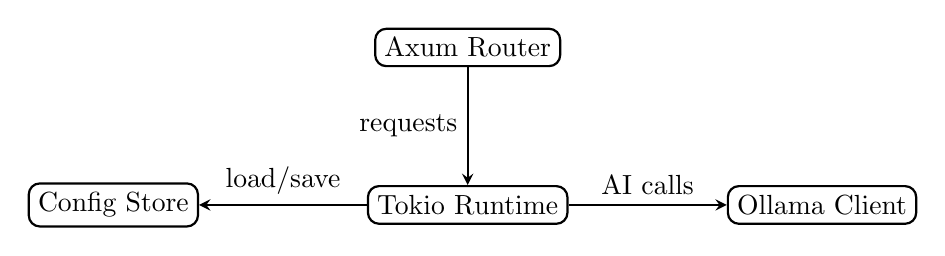
\begin{tikzpicture}[node distance=2cm,>=stealth,thick]
        \node (listener) [draw, rounded corners] {Axum Router};
        \node (runtime) [draw, rounded corners, below of=listener] {Tokio Runtime};
        \node (ai) [draw, rounded corners, right of=runtime, xshift=2.5cm] {Ollama Client};
        \node (cfg) [draw, rounded corners, left of=runtime, xshift=-2.5cm] {Config Store};
        \draw[->] (listener) -- node[left]{requests} (runtime);
        \draw[->] (runtime) -- node[above]{AI calls} (ai);
        \draw[->] (runtime) -- node[above]{load/save} (cfg);
    \end{tikzpicture}
    \caption{Axum handlers run inside the Tokio runtime, calling into AI and config subsystems asynchronously.}
\end{figure}

Minimal handler pattern:
\begin{verbatim}
#[derive(Deserialize)]
struct GoalBody { goal: Option<String> }

async fn propose(Json(body): Json<GoalBody>) -> Result<String, ApiError> {
    let goal = body.goal.unwrap_or("balanced".into());
    let plan = ai.propose_profile(&goal, Some(snapshot)).await?;
    Ok(plan)
}
\end{verbatim}

\section{Data Formats (Serde/TOML/JSON)}
\begin{itemize}
    \item Config persists to TOML via \texttt{serde} and \texttt{toml}.
    \item API responses use JSON automatically via Axum's \texttt{Json} extractor.
    \item Enable Serde features on external types (e.g., \texttt{uuid}).
\end{itemize}

\section{Error Handling}
\begin{itemize}
    \item Use \texttt{anyhow::Result} for binary entrypoints.
    \item Map errors to HTTP responses in handlers using a small helper (e.g., \texttt{internal\_error}).
    \item For library crates, prefer \texttt{thiserror} for typed errors.
\end{itemize}

\section{Testing Patterns}
\begin{itemize}
    \item Unit test prompt builders and config validators.
    \item Spin up Axum router with \texttt{tower::ServiceExt} for integration tests.
    \item Use \texttt{tokio::test} for async cases.
\end{itemize}

\section{Moving Forward}
After this primer, you should be comfortable reading the Smart Relay source, extending handlers, and integrating real proxy adapters.


\chapter{Proxy and VPN Clients}

\section{Comparing Clients}
Traditional clients like v2rayN are powerful but require manual rule curation. Smart Relay aims to keep the power while automating decisions with AI.

\section{Control vs Data Plane}
The control plane decides routes and pushes configs to the data plane engines (xray, sing-box). Smart Relay ships adapters to bridge the decision layer to the engines.

\section{Example Deployment Topology}
\begin{figure}[h]
    \centering
    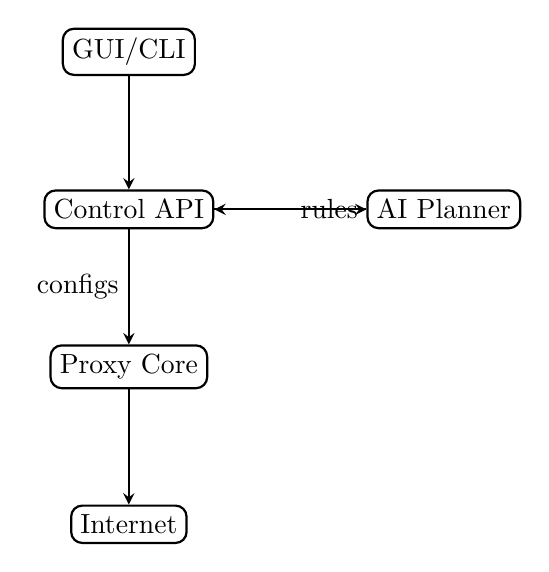
\begin{tikzpicture}[node distance=2cm,>=stealth,thick]
        \node (ui) [draw, rounded corners] {GUI/CLI};
        \node (api) [draw, rounded corners, below of=ui] {Control API};
        \node (ai) [draw, rounded corners, right of=api, xshift=2cm] {AI Planner};
        \node (core) [draw, rounded corners, below of=api] {Proxy Core};
        \node (internet) [draw, rounded corners, below of=core] {Internet};
        \draw[->] (ui) -- (api);
        \draw[->] (api) -- (ai);
        \draw[->] (ai) -- node[right]{rules} (api);
        \draw[->] (api) -- node[left]{configs} (core);
        \draw[->] (core) -- (internet);
    \end{tikzpicture}
    \caption{Control plane automates decisions; data plane forwards traffic.}
\end{figure}

\section{Key Features for a Modern Client}
\begin{itemize}
    \item Health-aware routing based on live probes.
    \item Zero-trust posture with minimal local secrets.
    \item First-class API for GUI, mobile, and scripting.
\end{itemize}

\section{Routing Strategies You Should Know}
\begin{itemize}
    \item \textbf{Geo-biasing}: steer video to low-latency regions, bulk downloads to cheapest egress.
    \item \textbf{Fail-open vs fail-closed}: pick policy per app; corporate traffic likely fail-closed.
    \item \textbf{Split tunneling}: only proxy destinations that need it; measure MTU/PMTU to avoid fragmentation.
    \item \textbf{Multi-hop}: optional double proxy for censorship-heavy regions; watch compounded latency.
\end{itemize}

\section{Core Integration Notes}
Start with a thin adapter that writes xray/sing-box JSON, validates it, then hot-reloads. Keep adapters isolated so UI/API never depends on a specific core schema.

\section{Suggested Checklists}
\begin{itemize}
    \item Preflight: DNS reachability, clock sync, certificate presence.
    \item Runtime: probe endpoints every N seconds, update scores, adjust weights.
    \item Postmortem: capture last applied config, probe logs, and AI rationale.
\end{itemize}


\chapter{Understanding VPNs: From Theory to Practice}

This chapter provides a comprehensive deep dive into Virtual Private Networks (VPNs), exploring how they work at different layers of the network stack, the protocols they use, and how they integrate with system networking. This knowledge is essential for understanding why endpoint testing requires multiple approaches and how Smart Relay orchestrates VPN connections.

\section{What is a VPN?}

A Virtual Private Network (VPN) creates a secure, encrypted tunnel between your device and a remote server, making it appear as if your network traffic originates from the VPN server rather than your actual location. This provides:

\begin{itemize}
    \item \textbf{Privacy}: Your real IP address is hidden from websites and services.
    \item \textbf{Security}: Traffic is encrypted, protecting it from interception.
    \item \textbf{Geographic flexibility}: Access content restricted to specific regions.
    \item \textbf{Network isolation}: Create private networks over public infrastructure.
\end{itemize}

\section{The OSI Model and VPN Layers}

VPNs operate at multiple layers of the OSI (Open Systems Interconnection) model. Understanding these layers helps diagnose connection issues and design better testing strategies.

\subsection{Layer 1-2: Physical and Data Link}

At the lowest layers, VPNs don't directly operate, but they rely on:
\begin{itemize}
    \item \textbf{Physical Layer (Layer 1)}: The actual network cables, wireless signals, and hardware.
    \item \textbf{Data Link Layer (Layer 2)}: Ethernet frames, MAC addresses, and local network protocols.
\end{itemize}

VPNs typically start their work at Layer 3 (Network) or higher.

\subsection{Layer 3: Network Layer (IP)}

The Network Layer is where IP (Internet Protocol) operates. This is where routing decisions are made and where many VPN protocols begin their work.

\begin{figure}[h]
    \centering
    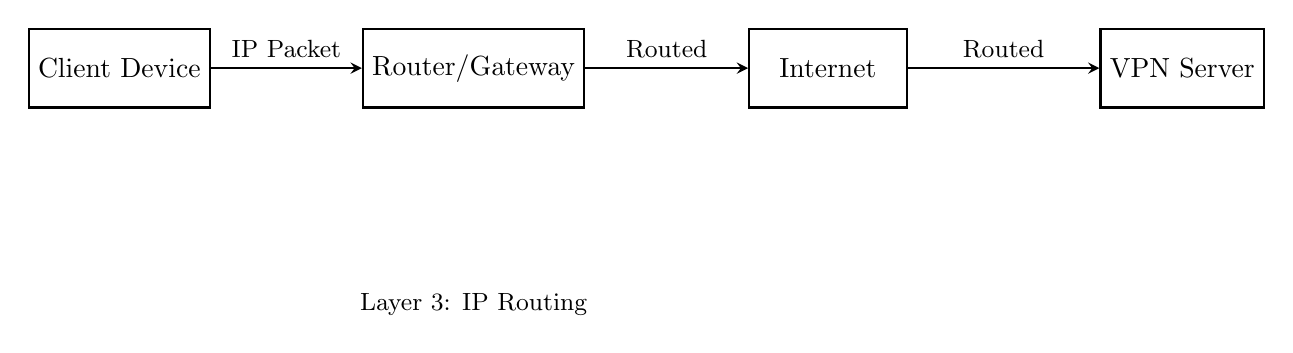
\begin{tikzpicture}[node distance=2.5cm,>=stealth,thick]
        \node (client) [draw, rectangle, minimum width=2cm, minimum height=1cm] {Client Device};
        \node (router) [draw, rectangle, minimum width=2cm, minimum height=1cm, right of=client, xshift=2cm] {Router/Gateway};
        \node (internet) [draw, rectangle, minimum width=2cm, minimum height=1cm, right of=router, xshift=2cm] {Internet};
        \node (vpn) [draw, rectangle, minimum width=2cm, minimum height=1cm, right of=internet, xshift=2cm] {VPN Server};
        
        \draw[->] (client) -- node[above]{\small IP Packet} (router);
        \draw[->] (router) -- node[above]{\small Routed} (internet);
        \draw[->] (internet) -- node[above]{\small Routed} (vpn);
        
        \node [below of=router, yshift=-0.5cm] {\small Layer 3: IP Routing};
    \end{tikzpicture}
    \caption{Network Layer (Layer 3) routing without VPN.}
\end{figure}

\textbf{Key concepts:}
\begin{itemize}
    \item \textbf{IP Addresses}: Unique identifiers for devices on the network (e.g., 192.168.1.100, 8.8.8.8).
    \item \textbf{Routing}: The process of forwarding packets from source to destination.
    \item \textbf{Subnetting}: Dividing networks into smaller subnetworks.
    \item \textbf{ICMP}: Internet Control Message Protocol for error reporting and diagnostics (ping uses ICMP).
\end{itemize}

\subsection{Layer 4: Transport Layer (TCP/UDP)}

The Transport Layer provides end-to-end communication services. This is where TCP (Transmission Control Protocol) and UDP (User Datagram Protocol) operate.

\begin{figure}[h]
    \centering
    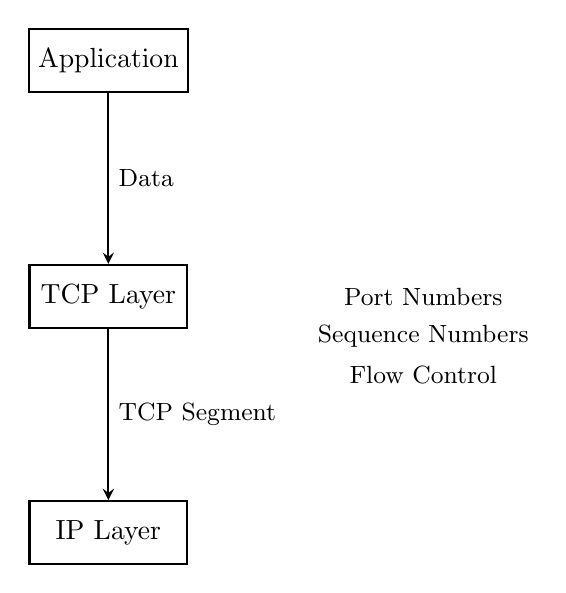
\begin{tikzpicture}[node distance=3cm,>=stealth,thick]
        \node (app) [draw, rectangle, minimum width=2cm, minimum height=0.8cm] {Application};
        \node (tcp) [draw, rectangle, minimum width=2cm, minimum height=0.8cm, below of=app] {TCP Layer};
        \node (ip) [draw, rectangle, minimum width=2cm, minimum height=0.8cm, below of=tcp] {IP Layer};
        
        \draw[->] (app) -- node[right]{\small Data} (tcp);
        \draw[->] (tcp) -- node[right]{\small TCP Segment} (ip);
        
        \node [right of=tcp, xshift=1cm] {\small Port Numbers};
        \node [right of=tcp, xshift=1cm, yshift=-0.5cm] {\small Sequence Numbers};
        \node [right of=tcp, xshift=1cm, yshift=-1cm] {\small Flow Control};
    \end{tikzpicture}
    \caption{Transport Layer (Layer 4) adds port numbers and reliability.}
\end{figure}

\textbf{TCP Three-Way Handshake:}
\begin{enumerate}
    \item \textbf{SYN}: Client sends a synchronization packet with a random sequence number.
    \item \textbf{SYN-ACK}: Server responds with its own sequence number and acknowledges the client's.
    \item \textbf{ACK}: Client acknowledges the server's sequence number. Connection established.
\end{enumerate}

\begin{figure}[h]
    \centering
    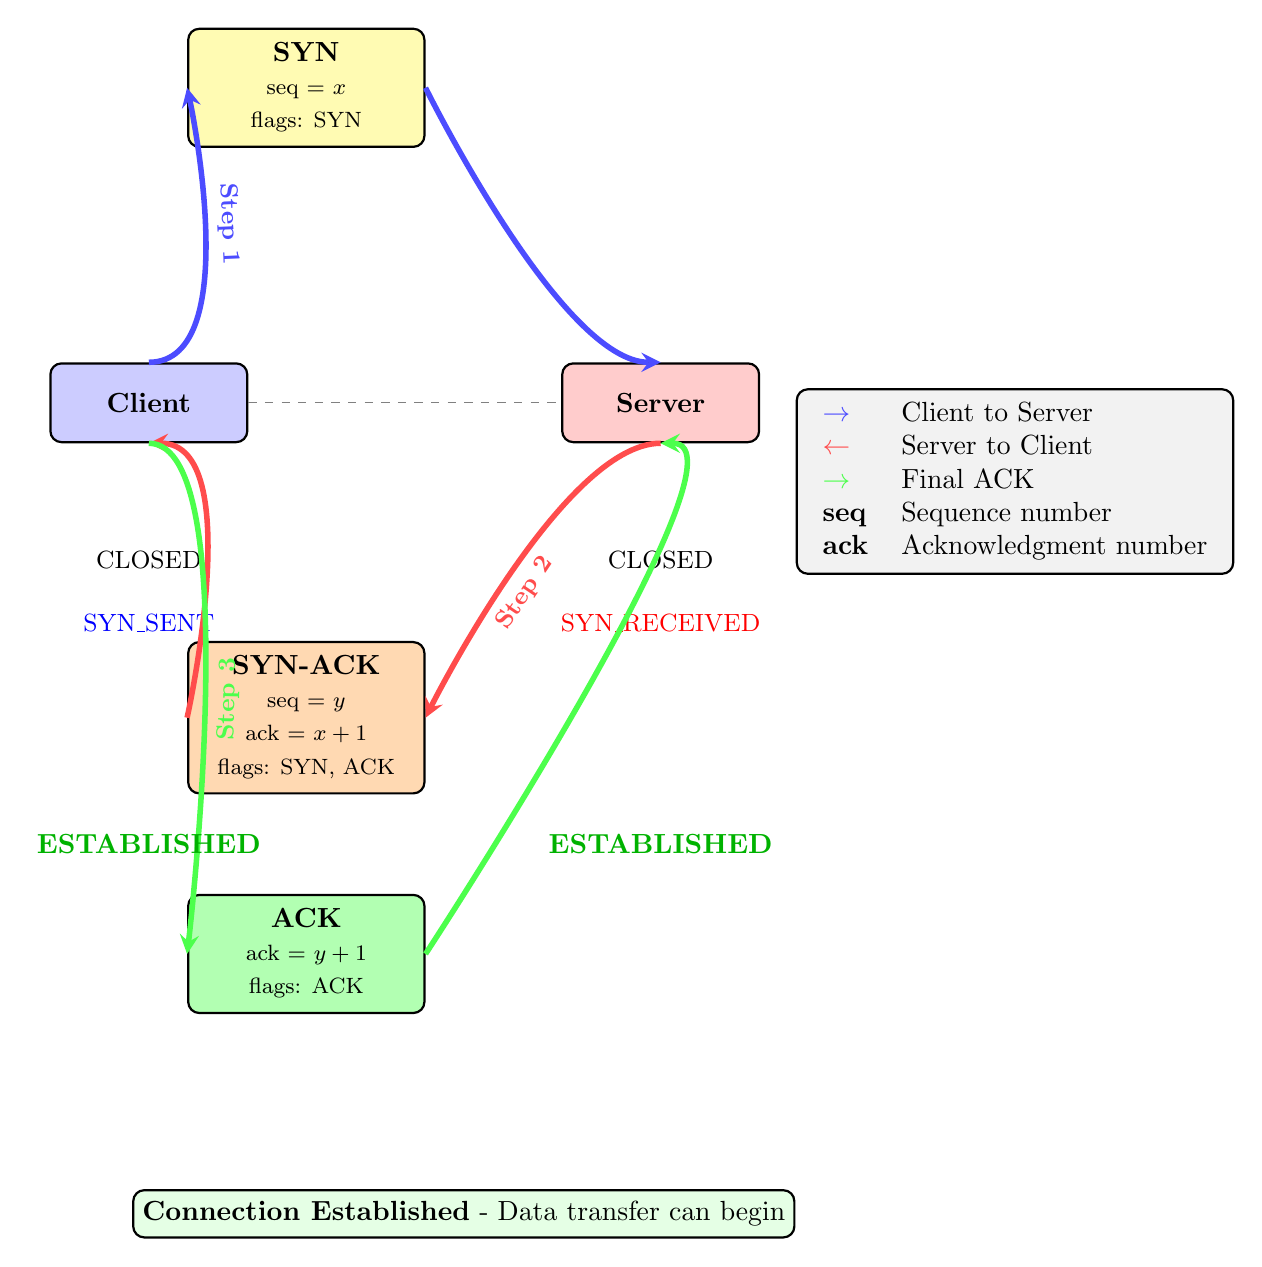
\begin{tikzpicture}[
        node distance=2.5cm,
        >=stealth,
        thick,
        state/.style={draw, rectangle, rounded corners, minimum width=2.5cm, minimum height=1cm, fill=blue!10},
        packet/.style={draw, rectangle, rounded corners, minimum width=3cm, minimum height=0.8cm, fill=green!20},
        arrow/.style={->, line width=2pt},
        timeline/.style={dashed, gray, line width=0.5pt}
    ]
        % Client and Server nodes
        \node (client) [state, fill=blue!20] {\textbf{Client}};
        \node (server) [state, fill=red!20, right of=client, xshift=4cm] {\textbf{Server}};
        
        % Connection states
        \node (client_closed) [below of=client, yshift=0.5cm, font=\small] {CLOSED};
        \node (server_closed) [below of=server, yshift=0.5cm, font=\small] {CLOSED};
        
        % Timeline
        \draw[timeline] (client) -- (server);
        
        % Step 1: SYN
        \node (syn_packet) [packet, fill=yellow!30, above of=client, yshift=1.5cm, xshift=2cm] {
            \begin{tabular}{c}
                \textbf{SYN} \\
                \footnotesize seq = $x$ \\
                \footnotesize flags: SYN
            \end{tabular}
        };
        \draw[arrow, blue!70] (client.north) .. controls (client.north east) and (syn_packet.west) .. 
            node[above, sloped, font=\small] {\textbf{Step 1}} (syn_packet.west);
        \draw[arrow, blue!70] (syn_packet.east) .. controls (syn_packet.east) and (server.north west) .. (server.north);
        
        \node (client_syn_sent) [below of=client, yshift=-0.3cm, font=\small, text=blue] {SYN\_SENT};
        
        % Step 2: SYN-ACK
        \node (synack_packet) [packet, fill=orange!30, below of=client, yshift=-1.5cm, xshift=2cm] {
            \begin{tabular}{c}
                \textbf{SYN-ACK} \\
                \footnotesize seq = $y$ \\
                \footnotesize ack = $x+1$ \\
                \footnotesize flags: SYN, ACK
            \end{tabular}
        };
        \draw[arrow, red!70] (server.south) .. controls (server.south west) and (synack_packet.east) .. 
            node[below, sloped, font=\small] {\textbf{Step 2}} (synack_packet.east);
        \draw[arrow, red!70] (synack_packet.west) .. controls (synack_packet.west) and (client.south east) .. (client.south);
        
        \node (server_syn_rcvd) [below of=server, yshift=-0.3cm, font=\small, text=red] {SYN\_RECEIVED};
        
        % Step 3: ACK
        \node (ack_packet) [packet, fill=green!30, below of=synack_packet, yshift=-0.5cm] {
            \begin{tabular}{c}
                \textbf{ACK} \\
                \footnotesize ack = $y+1$ \\
                \footnotesize flags: ACK
            \end{tabular}
        };
        \draw[arrow, green!70] (client.south) .. controls (client.south east) and (ack_packet.west) .. 
            node[below, sloped, font=\small] {\textbf{Step 3}} (ack_packet.west);
        \draw[arrow, green!70] (ack_packet.east) .. controls (ack_packet.east) and (server.south east) .. (server.south);
        
        % Established state
        \node (client_est) [below of=client_syn_sent, yshift=-0.3cm, font=\small, text=green!70!black, font=\bfseries] {ESTABLISHED};
        \node (server_est) [below of=server_syn_rcvd, yshift=-0.3cm, font=\small, text=green!70!black, font=\bfseries] {ESTABLISHED};
        
        % Connection established indicator
        \node (established) [draw, rectangle, rounded corners, fill=green!10, minimum width=6cm, minimum height=0.6cm, 
            below of=ack_packet, yshift=-0.8cm, xshift=2cm] {
            \textbf{Connection Established} - Data transfer can begin
        };
        
        % Legend
        \node (legend) [draw, rectangle, rounded corners, fill=gray!10, minimum width=5cm, minimum height=2cm,
            right of=server, xshift=2cm, yshift=-1cm] {
            \begin{tabular}{ll}
                \textcolor{blue!70}{$\rightarrow$} & Client to Server \\
                \textcolor{red!70}{$\leftarrow$} & Server to Client \\
                \textcolor{green!70}{$\rightarrow$} & Final ACK \\
                \textbf{seq} & Sequence number \\
                \textbf{ack} & Acknowledgment number \\
            \end{tabular}
        };
    \end{tikzpicture}
    \caption{TCP three-way handshake process with detailed packet information and state transitions.}
\end{figure}
\textbf{Why this matters for VPN testing:}
\begin{itemize}
    \item If SYN packets are sent but no SYN-ACK is received, the connection fails at Layer 4.
    \item Firewalls often drop SYN packets silently (stealth mode), causing timeouts.
    \item Connection refused errors indicate the port is closed (RST packet received).
    \item Timeouts suggest packets are being dropped or not routed correctly.
\end{itemize}

\subsection{Layer 5-7: Session, Presentation, Application}

Higher layers handle:
\begin{itemize}
    \item \textbf{Session Layer (Layer 5)}: Manages sessions between applications.
    \item \textbf{Presentation Layer (Layer 6)}: Data translation, encryption, compression.
    \item \textbf{Application Layer (Layer 7)}: HTTP, HTTPS, DNS, FTP, and application protocols.
\end{itemize}

VPN protocols often operate at these layers, encapsulating lower-layer traffic.

\section{VPN Tunneling Mechanisms}

VPNs create "tunnels" by encapsulating one protocol within another. This section explains the different tunneling approaches.

\subsection{IP-in-IP Tunneling}

The simplest form of tunneling: one IP packet is placed inside another IP packet.

\begin{figure}[h]
    \centering
    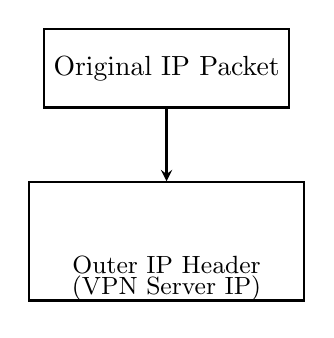
\begin{tikzpicture}[node distance=2cm,>=stealth,thick]
        \node (original) [draw, rectangle, minimum width=3cm, minimum height=1cm] {Original IP Packet};
        \node (encapsulated) [draw, rectangle, minimum width=3.5cm, minimum height=1.5cm, below of=original, yshift=-0.2cm] {};
        \node [below of=original, yshift=-0.5cm] {\small Outer IP Header};
        \node [below of=original, yshift=-0.8cm] {\small (VPN Server IP)};
        
        \draw[->] (original) -- (encapsulated);
    \end{tikzpicture}
    \caption{IP-in-IP encapsulation: original packet wrapped in new IP header.}
\end{figure}

\textbf{How it works:}
\begin{enumerate}
    \item Original packet has destination IP of the final target.
    \item VPN client wraps it in a new IP packet with destination of VPN server.
    \item VPN server unwraps and forwards the original packet.
    \item Response follows the reverse path.
\end{enumerate}

\subsection{Protocol-Specific Tunneling}

Different VPN protocols use different encapsulation methods:

\subsubsection{OpenVPN}
\begin{itemize}
    \item Uses UDP or TCP for transport.
    \item Encapsulates IP packets in OpenVPN protocol.
    \item Supports both TUN (Layer 3) and TAP (Layer 2) modes.
    \item Uses TLS/SSL for key exchange and authentication.
\end{itemize}

\subsubsection{WireGuard}
\begin{itemize}
    \item Modern, lightweight VPN protocol.
    \item Uses UDP for transport.
    \item Operates at Layer 3 (IP level).
    \item Uses state-of-the-art cryptography (ChaCha20, Poly1305, Curve25519).
\end{itemize}

\subsubsection{IPSec}
\begin{itemize}
    \item Operates at Layer 3 (Network Layer).
    \item Can work in two modes:
    \begin{itemize}
        \item \textbf{Transport Mode}: Encrypts only the payload.
        \item \textbf{Tunnel Mode}: Encrypts the entire IP packet.
    \end{itemize}
    \item Often used for site-to-site VPNs.
\end{itemize}

\subsubsection{Shadowsocks, VMess, VLESS (Proxy Protocols)}
\begin{itemize}
    \item These are proxy protocols, not traditional VPNs.
    \item Operate at Layer 5-7 (Application/Session layers).
    \item Encrypt and forward application-layer traffic (HTTP, HTTPS, etc.).
    \item Don't create a true network interface like traditional VPNs.
    \item Work by intercepting application traffic and forwarding it through a proxy server.
\end{itemize}

\section{How VPNs Integrate with Operating Systems}

Understanding how VPNs hook into the operating system is crucial for implementing system proxy integration.

\subsection{Network Interface Creation}

Traditional VPNs create virtual network interfaces:

\begin{figure}[h]
    \centering
    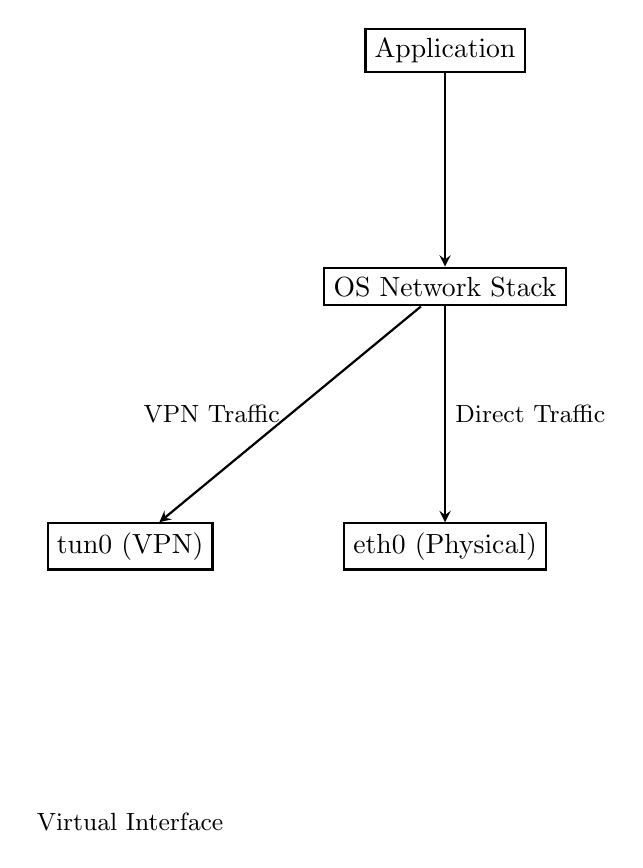
\begin{tikzpicture}[node distance=3cm,>=stealth,thick]
        \node (app) [draw, rectangle, minimum width=2cm] {Application};
        \node (os) [draw, rectangle, minimum width=2cm, below of=app] {OS Network Stack};
        \node (eth0) [draw, rectangle, minimum width=2cm, below of=os, yshift=-0.3cm] {eth0 (Physical)};
        \node (tun0) [draw, rectangle, minimum width=2cm, left of=eth0, xshift=-1cm] {tun0 (VPN)};
        
        \draw[->] (app) -- (os);
        \draw[->] (os) -- node[left]{\small VPN Traffic} (tun0);
        \draw[->] (os) -- node[right]{\small Direct Traffic} (eth0);
        
        \node [below of=tun0, yshift=-0.5cm] {\small Virtual Interface};
    \end{tikzpicture}
    \caption{VPN creates virtual network interface (tun0/tap0).}
\end{figure}

\textbf{On different operating systems:}
\begin{itemize}
    \item \textbf{Linux}: Creates \texttt{tun0} or \texttt{tap0} interfaces.
    \item \textbf{Windows}: Creates TAP adapters (visible in Network Connections).
    \item \textbf{macOS}: Creates \texttt{utun} interfaces.
\end{itemize}

\subsection{Routing Table Modification}

VPNs modify the routing table to direct traffic through the VPN interface:

\begin{verbatim}
# Example routing table with VPN active
Destination     Gateway         Genmask         Flags Interface
0.0.0.0         10.8.0.1        0.0.0.0         UG    tun0    # Default via VPN
10.8.0.0        0.0.0.0         255.255.255.0   U     tun0    # VPN subnet
192.168.1.0     0.0.0.0         255.255.255.0   U     eth0    # Local network
\end{verbatim}

\subsection{Proxy vs. VPN: System Integration}

\subsubsection{Traditional VPN (TUN/TAP)}
\begin{itemize}
    \item Creates a virtual network interface.
    \item Modifies routing table.
    \item All IP traffic can be routed through VPN.
    \item Transparent to applications (they don't know VPN exists).
    \item Examples: OpenVPN, WireGuard, IPSec.
\end{itemize}

\subsubsection{Proxy-Based (Application Layer)}
\begin{itemize}
    \item No virtual network interface.
    \item Applications must be configured to use proxy.
    \item Only configured applications use proxy.
    \item System proxy settings tell applications where to connect.
    \item Examples: Shadowsocks, VMess, VLESS, SOCKS5, HTTP proxy.
\end{itemize}

\begin{figure}[h]
    \centering
    \begin{tikzpicture}[node distance=3cm,>=stealth,thick]
        \node (app1) [draw, rectangle, minimum width=1.5cm] {App 1};
        \node (app2) [draw, rectangle, minimum width=1.5cm, below of=app1] {App 2};
        \node (proxy) [draw, rectangle, minimum width=2cm, right of=app1, xshift=1cm] {Proxy Client};
        \node (server) [draw, rectangle, minimum width=2cm, right of=proxy, xshift=1cm] {Proxy Server};
        
        \draw[->] (app1) -- node[above]{\small Configured} (proxy);
        \draw[->] (app2) -- node[below]{\small Direct} ++(2,0);
        \draw[->] (proxy) -- node[above]{\small Encrypted} (server);
        
        \node [below of=app2, yshift=-0.5cm] {\small Not using proxy};
    \end{tikzpicture}
    \caption{Proxy-based VPN: only configured applications use it.}
\end{figure}

\section{Windows System Proxy Integration}

Smart Relay uses Windows system proxy settings to route application traffic through proxy servers. Understanding how this works is essential.

\subsection{Windows Proxy Registry Keys}

Windows stores proxy settings in the registry:

\begin{verbatim}
HKEY_CURRENT_USER\Software\Microsoft\Windows\CurrentVersion\Internet Settings
\end{verbatim}

\textbf{Key values:}
\begin{itemize}
    \item \texttt{ProxyEnable}: 1 = proxy enabled, 0 = disabled.
    \item \texttt{ProxyServer}: Format: \texttt{host:port} or \texttt{http=host:port;https=host:port;ftp=host:port;socks=host:port}
    \item \texttt{ProxyOverride}: Semicolon-separated list of addresses that bypass proxy.
    \item \texttt{AutoConfigURL}: URL to PAC (Proxy Auto-Configuration) script.
\end{itemize}

\subsection{Global Proxy Mode}

In Global mode, all HTTP/HTTPS traffic goes through the specified proxy:

\begin{figure}[h]
    \centering
    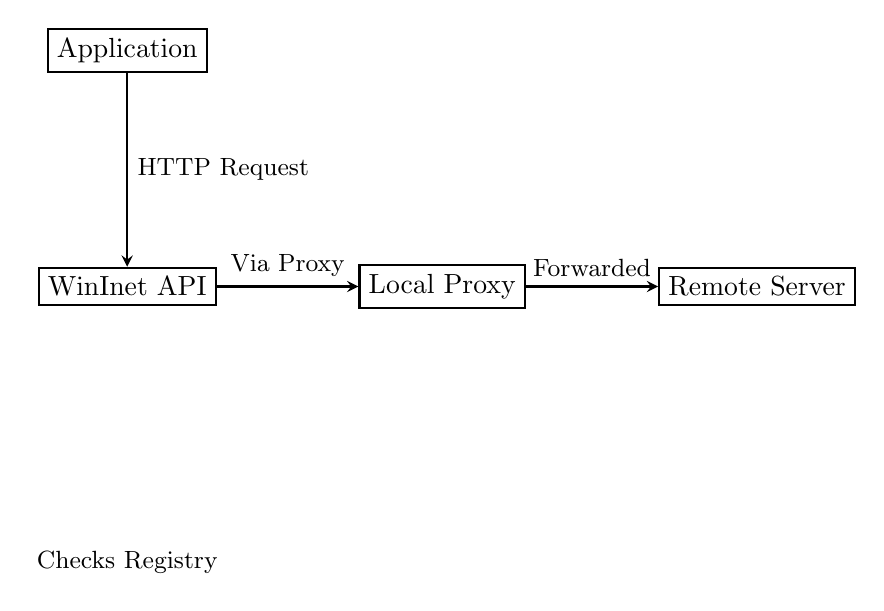
\begin{tikzpicture}[node distance=3cm,>=stealth,thick]
        \node (app) [draw, rectangle, minimum width=2cm] {Application};
        \node (wininet) [draw, rectangle, minimum width=2cm, below of=app] {WinInet API};
        \node (proxy) [draw, rectangle, minimum width=2cm, right of=wininet, xshift=1cm] {Local Proxy};
        \node (server) [draw, rectangle, minimum width=2cm, right of=proxy, xshift=1cm] {Remote Server};
        
        \draw[->] (app) -- node[right]{\small HTTP Request} (wininet);
        \draw[->] (wininet) -- node[above]{\small Via Proxy} (proxy);
        \draw[->] (proxy) -- node[above]{\small Forwarded} (server);
        
        \node [below of=wininet, yshift=-0.5cm] {\small Checks Registry};
    \end{tikzpicture}
    \caption{Global proxy mode: WinInet routes all HTTP/HTTPS through proxy.}
\end{figure}

\textbf{How it works:}
\begin{enumerate}
    \item Application makes HTTP/HTTPS request using WinInet API.
    \item WinInet checks registry for \texttt{ProxyEnable} and \texttt{ProxyServer}.
    \item If enabled, WinInet connects to proxy instead of destination.
    \item Proxy forwards request to actual destination.
    \item Response follows reverse path.
\end{enumerate}

\subsection{PAC (Proxy Auto-Configuration) Mode}

PAC mode uses a JavaScript file to dynamically determine proxy settings:

\begin{verbatim}
function FindProxyForURL(url, host) {
    if (isPlainHostName(host) || 
        dnsDomainIs(host, ".local") ||
        isInNet(host, "192.168.0.0", "255.255.0.0")) {
        return "DIRECT";
    }
    return "PROXY 127.0.0.1:1080; SOCKS5 127.0.0.1:1080";
}
\end{verbatim}

\textbf{Benefits:}
\begin{itemize}
    \item Different proxies for different domains.
    \item Bypass proxy for local addresses.
    \item Load balancing across multiple proxies.
    \item Dynamic configuration without registry changes.
\end{itemize}

\subsection{Limitations of System Proxy}

\begin{itemize}
    \item \textbf{Application support}: Only applications using WinInet API respect system proxy.
    \item \textbf{Non-HTTP traffic}: System proxy typically only handles HTTP/HTTPS, not raw TCP/UDP.
    \item \textbf{Administrator rights}: Some proxy operations may require elevated privileges.
    \item \textbf{Bypass mechanisms}: Some applications have hardcoded proxy bypasses.
\end{itemize}

\section{Why Endpoint Testing is Complex}

Now that we understand VPNs and networking layers, we can see why comprehensive endpoint testing requires multiple approaches.

\subsection{The Testing Challenge}

When testing a VPN endpoint, we need to verify:

\begin{enumerate}
    \item \textbf{DNS Resolution (Layer 7)}: Can we resolve the hostname?
    \item \textbf{Network Reachability (Layer 3)}: Can we route packets to the server?
    \item \textbf{Port Accessibility (Layer 4)}: Is the port open and accepting connections?
    \item \textbf{Protocol Compatibility (Layer 5-7)}: Does the protocol work correctly?
    \item \textbf{Proxy Functionality (Layer 5-7)}: Can we actually use it as a proxy?
\end{enumerate}

\subsection{Why Direct TCP Tests May Fail}

A direct TCP connection test might fail even if the endpoint works through a proxy:

\begin{itemize}
    \item \textbf{Firewall blocking}: The server may only accept connections from specific IPs (e.g., only from other VPN servers).
    \item \textbf{Protocol requirement}: Some protocols (like VMess) require specific handshakes that a simple TCP test can't perform.
    \item \textbf{Rate limiting}: Servers may rate-limit direct connections but allow proxy connections.
    \item \textbf{Geographic restrictions}: The server may block direct connections from certain regions.
\end{itemize}

\subsection{Why Proxy Tests May Fail}

Testing through a local proxy may also fail:

\begin{itemize}
    \item \textbf{Local proxy not running}: The proxy client (xray, sing-box) must be running and configured.
    \item \textbf{Configuration mismatch}: The proxy client may not be configured to use the endpoint being tested.
    \item \textbf{Protocol incompatibility}: The local proxy may not support the endpoint's protocol.
    \item \textbf{Authentication failure}: Credentials or encryption keys may be incorrect.
\end{itemize}

\subsection{Smart Testing Strategy}

Smart Relay's comprehensive testing approach:

\begin{enumerate}
    \item \textbf{DNS Resolution}: Verify hostname can be resolved (Layer 7).
    \item \textbf{Direct TCP Connection}: Attempt direct connection (Layer 4).
    \begin{itemize}
        \item If successful: Endpoint is reachable.
        \item If failed: May still work through proxy.
    \end{itemize}
    \item \textbf{Proxy-Based Test}: If local proxy is available, test through it (Layer 5-7).
    \item \textbf{Extended Timeout}: Some connections are slow but work (Layer 4).
    \item \textbf{Diagnostic Analysis}: Categorize failures to provide actionable feedback.
\end{enumerate}

\section{Packet-Level Analysis}

Understanding what happens at the packet level helps diagnose connection issues.

\subsection{TCP Packet Structure}

A TCP packet contains:

\begin{verbatim}
+-------------------+-------------------+
| Source Port (16)  | Dest Port (16)    |
+-------------------+-------------------+
| Sequence Number (32 bits)              |
+---------------------------------------+
| Acknowledgment Number (32 bits)       |
+-------+-------+-----------------------+
| Data  | Flags | Window Size (16)      |
|Offset |(SYN,  |                       |
| (4)   |ACK...)|                       |
+-------+-------+-----------------------+
| Checksum (16)    | Urgent Pointer (16)|
+------------------+--------------------+
| Options (variable length)             |
+---------------------------------------+
| Data (variable length)                |
+---------------------------------------+
\end{verbatim}

\subsection{Connection States}

TCP connections go through several states:

\begin{itemize}
    \item \textbf{CLOSED}: No connection exists.
    \item \textbf{SYN\_SENT}: Client sent SYN, waiting for SYN-ACK.
    \item \textbf{SYN\_RECEIVED}: Server received SYN, sent SYN-ACK, waiting for ACK.
    \item \textbf{ESTABLISHED}: Connection is open and data can be exchanged.
    \item \textbf{FIN\_WAIT}: Connection is being closed.
    \item \textbf{CLOSED}: Connection is fully closed.
\end{itemize}

\subsection{Error Scenarios}

\begin{itemize}
    \item \textbf{Connection Refused (RST)}:
    \begin{itemize}
        \item Server received SYN.
        \item Server sent RST (reset) packet.
        \item Port is closed or service not running.
    \end{itemize}
    
    \item \textbf{Connection Timeout}:
    \begin{itemize}
        \item Client sent SYN.
        \item No response received (SYN-ACK or RST).
        \item Firewall dropping packets silently.
        \item Network routing issue.
        \item Server is down or unreachable.
    \end{itemize}
    
    \item \textbf{Network Unreachable}:
    \begin{itemize}
        \item No route to destination.
        \item ICMP "Destination Unreachable" may be received.
        \item Network configuration issue.
    \end{itemize}
\end{itemize}

\section{Practical Implications for Smart Relay}

This deep understanding of VPNs and networking informs Smart Relay's design:

\begin{itemize}
    \item \textbf{Multi-layer testing}: Test at DNS, TCP, and proxy levels.
    \item \textbf{Comprehensive diagnostics}: Provide detailed information about failures.
    \item \textbf{System integration}: Use Windows registry for proxy configuration.
    \item \textbf{Protocol support}: Handle both traditional VPNs and proxy protocols.
    \item \textbf{Error categorization}: Help users understand what went wrong.
\end{itemize}

\section{Understanding Network Censorship and Firewalls}

Understanding how network firewalls and censorship systems work helps explain why endpoints may fail even when you're outside restricted regions. This section discusses the technical principles behind network filtering systems.

\subsection{Multi-Layer Filtering}

Network filtering systems can operate at multiple OSI layers:

\begin{figure}[h]
    \centering
    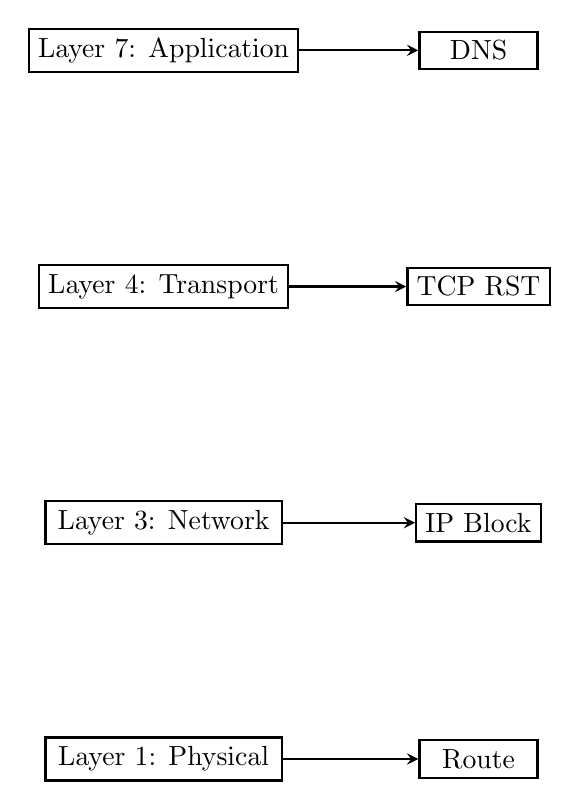
\begin{tikzpicture}[node distance=3cm,>=stealth,thick]
        \node (layer7) [draw, rectangle, minimum width=3cm] {Layer 7: Application};
        \node (layer4) [draw, rectangle, minimum width=3cm, below of=layer7] {Layer 4: Transport};
        \node (layer3) [draw, rectangle, minimum width=3cm, below of=layer4] {Layer 3: Network};
        \node (layer1) [draw, rectangle, minimum width=3cm, below of=layer3] {Layer 1: Physical};
        
        \node (dns) [draw, rectangle, minimum width=1.5cm, right of=layer7, xshift=1cm] {DNS};
        \node (tcp) [draw, rectangle, minimum width=1.5cm, right of=layer4, xshift=1cm] {TCP RST};
        \node (ip) [draw, rectangle, minimum width=1.5cm, right of=layer3, xshift=1cm] {IP Block};
        \node (route) [draw, rectangle, minimum width=1.5cm, right of=layer1, xshift=1cm] {Route};
        
        \draw[->] (layer7) -- (dns);
        \draw[->] (layer4) -- (tcp);
        \draw[->] (layer3) -- (ip);
        \draw[->] (layer1) -- (route);
    \end{tikzpicture}
    \caption{Network filtering can occur at multiple OSI layers.}
\end{figure}

\subsection{DNS Pollution and Hijacking}

\textbf{How it works:}
\begin{itemize}
    \item DNS queries are typically unencrypted (plaintext).
    \item When a DNS query for a blocked domain is detected, the firewall intercepts it.
    \item Instead of forwarding to the real DNS server, it returns a fake IP address.
    \item This is called "DNS pollution" or "DNS hijacking."
\end{itemize}

\textbf{Why it's effective:}
\begin{itemize}
    \item Very resource-efficient (minimal network overhead).
    \item Blocks most users who don't understand DNS.
    \item Works before any connection is established.
\end{itemize}

\textbf{How to detect:}
\begin{itemize}
    \item Compare DNS results from different DNS servers (8.8.8.8, 1.1.1.1).
    \item Use encrypted DNS (DNS over HTTPS/TLS).
    \item Check if resolved IPs are actually reachable.
\end{itemize}

\subsection{IP and Port Blocking}

\textbf{Route Nullification (Blackhole Routing):}
\begin{itemize}
    \item Firewalls can configure routers to drop packets to specific IP addresses.
    \item This is done by creating "null routes" or "blackhole routes."
    \item Packets are routed to a "blackhole" interface that discards them.
    \item Very efficient: packets are dropped before leaving the local network.
    \item This is why some IPs are unreachable even though DNS resolution works.
\end{itemize}

\textbf{Port Blocking:}
\begin{itemize}
    \item Specific ports (e.g., common VPN ports) can be blocked.
    \item Often combined with IP blocking for comprehensive filtering.
    \item Some firewalls block entire IP ranges (e.g., all of Google's IPs).
\end{itemize}

\subsection{Deep Packet Inspection (DPI) and Protocol Recognition}

\textbf{Keyword Filtering:}
\begin{itemize}
    \item Firewalls can inspect unencrypted traffic (HTTP, FTP, SMTP).
    \item When forbidden keywords are detected, TCP RST packets are sent to both sides.
    \item This terminates the connection immediately.
    \item Works because these protocols send data in plaintext.
\end{itemize}

\textbf{Protocol Fingerprinting:}
\begin{itemize}
    \item Different protocols have distinct "fingerprints" (handshake patterns, packet sizes, timing).
    \item Firewalls can identify protocols even if content is encrypted:
    \begin{itemize}
        \item OpenVPN: Specific handshake pattern
        \item PPTP: Distinct packet structure
        \item HTTP Proxy: CONNECT method pattern
        \item SOCKS5: Specific handshake sequence
    \end{itemize}
    \item Once identified, connections can be blocked or throttled.
\end{itemize}

\textbf{TLS Fingerprinting:}
\begin{itemize}
    \item Even encrypted TLS connections have identifiable characteristics.
    \item TLS handshake includes unencrypted metadata (cipher suites, extensions).
    \item Some implementations have unique fingerprints.
    \item Vulnerabilities in specific versions can be exploited for detection.
\end{itemize}

\subsection{TCP Reset (RST) Attacks}

\textbf{How TCP RST works:}
\begin{itemize}
    \item When a firewall detects forbidden content or protocol:
    \begin{enumerate}
        \item Firewall sends TCP RST packet to client (spoofed as server).
        \item Firewall sends TCP RST packet to server (spoofed as client).
        \item Both sides think the other disconnected.
        \item Connection is terminated immediately.
    \end{enumerate}
    \item This is why you might see "Connection reset by peer" errors.
\end{itemize}

\textbf{Why it's effective:}
\begin{itemize}
    \item Works on established connections (not just new ones).
    \item Very fast (connection drops immediately).
    \item Hard to distinguish from legitimate connection failures.
\end{itemize}

\subsection{Why Endpoints May Fail Even Outside Restricted Regions}

Even if you're outside regions with network filtering, endpoints can still fail for several reasons:

\subsubsection{Server-Side Restrictions}

\begin{itemize}
    \item \textbf{Geographic IP Filtering}: Servers may only accept connections from specific regions.
    \item \textbf{Whitelist-Based Access}: Some VPN servers only allow connections from other VPN servers.
    \item \textbf{Rate Limiting}: Servers may block direct connections but allow proxy connections.
    \item \textbf{Port Restrictions}: Servers may only accept connections on specific ports or from specific IPs.
\end{itemize}

\subsubsection{Protocol Requirements}

\begin{itemize}
    \item \textbf{Protocol-Specific Handshakes}: VMess, Shadowsocks, and other protocols require specific handshakes.
    \item \textbf{Simple TCP tests fail}: A basic TCP connection test can't perform the required protocol handshake.
    \item \textbf{Authentication Required}: Many protocols require authentication before accepting connections.
    \item \textbf{Encryption Keys}: Connections may require specific encryption keys or certificates.
\end{itemize}

\subsubsection{Network Path Issues}

\begin{itemize}
    \item \textbf{Intermediate Firewalls}: Your ISP or intermediate networks may block certain IPs or ports.
    \item \textbf{Routing Problems}: Network routing issues can prevent packets from reaching the destination.
    \item \textbf{Server Downtime}: The endpoint server may be down or overloaded.
    \item \textbf{Maintenance}: Servers may be temporarily unavailable for maintenance.
\end{itemize}

\subsubsection{Why Direct TCP Tests Fail But Proxy Works}

This is a common scenario:

\begin{enumerate}
    \item \textbf{Direct TCP test fails}: Simple TCP connection to endpoint times out or is refused.
    \item \textbf{But proxy works}: When connecting through a properly configured proxy client, it works.
    
    \textbf{Why?}
    \begin{itemize}
        \item Server may only accept connections with proper protocol handshake (VMess, Shadowsocks, etc.).
        \item Server may require connections from specific IP ranges (other VPN servers).
        \item Server may rate-limit direct connections but allow proxy connections.
        \item The proxy client performs the required protocol handshake and authentication.
    \end{itemize}
\end{enumerate}

\subsection{Interpreting Diagnostic Results}

When you see connection failures, consider:

\begin{itemize}
    \item \textbf{DNS Resolution Works}: Hostname resolves to IP → DNS is not the problem.
    \item \textbf{Routing Works}: Traceroute shows packets are being routed → Network path exists.
    \item \textbf{TCP Connection Fails}: SYN sent but no SYN-ACK received → Possible causes:
    \begin{itemize}
        \item Firewall blocking (intermediate or server-side).
        \item Server not accepting direct TCP connections (requires protocol handshake).
        \item Port is closed or service is down.
        \item Geographic restrictions.
    \end{itemize}
    \item \textbf{Proxy Test Fails}: Local proxy not available → Need to start proxy client first.
\end{itemize}

\subsection{Best Practices for Endpoint Testing}

\begin{enumerate}
    \item \textbf{Test DNS First}: If DNS fails, nothing else matters.
    \item \textbf{Test Routing}: Verify packets can reach the destination network.
    \item \textbf{Test TCP}: Check if basic connectivity works.
    \item \textbf{Test Through Proxy}: If direct fails, test through properly configured proxy.
    \item \textbf{Check Protocol Requirements}: Ensure you're using the correct protocol and authentication.
    \item \textbf{Consider Geographic Restrictions}: Some endpoints may only work from specific regions.
\end{enumerate}

\section{Further Reading}

\begin{itemize}
    \item RFC 791: Internet Protocol (IP)
    \item RFC 793: Transmission Control Protocol (TCP)
    \item RFC 2661: Layer Two Tunneling Protocol (L2TP)
    \item WireGuard Protocol Documentation
    \item VMess Protocol Specification (V2Ray)
    \item Shadowsocks Protocol Documentation
    \item DNS over HTTPS (DoH) and DNS over TLS (DoT) specifications
    \item TLS Fingerprinting research papers
\end{itemize}


\chapter{AI-Driven Design with Ollama}

\section{Prompt Engineering}
Provide the AI with context: current endpoints, latency goals, blocked regions, and risk appetite. Keep prompts short; ask for structured bullet plans.

\section{Closed-Loop Automation}
\begin{figure}[h]
    \centering
    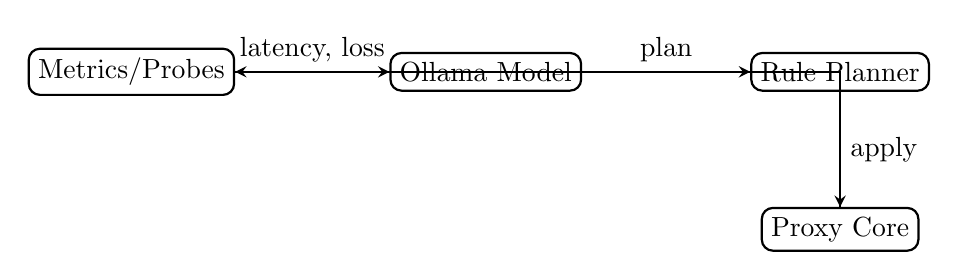
\begin{tikzpicture}[node distance=2cm,>=stealth,thick]
        \node (metrics) [draw, rounded corners] {Metrics/Probes};
        \node (ai) [draw, rounded corners, right of=metrics, xshift=2.5cm] {Ollama Model};
        \node (planner) [draw, rounded corners, right of=ai, xshift=2.5cm] {Rule Planner};
        \node (core) [draw, rounded corners, below of=planner] {Proxy Core};
        \draw[->] (metrics) -- node[above]{latency, loss} (ai);
        \draw[->] (ai) -- node[above]{plan} (planner);
        \draw[->] (planner) -- node[right]{apply} (core);
        \draw[->] (core) |- (metrics);
    \end{tikzpicture}
    \caption{Feedback loop keeps routes healthy and policies updated.}
\end{figure}

\section{Safety Rails}
\begin{itemize}
    \item Validate AI outputs before applying (schema + sandbox).
    \item Rate-limit reconfiguration to avoid flapping.
    \item Keep human-in-the-loop for sensitive regions.
\end{itemize}

\section{Prompt Patterns That Work Well}
\begin{itemize}
    \item \textbf{Structured bullets}: ask for ``Endpoints:``, ``Rules:``, ``Risks:`` sections.
    \item \textbf{Constraints}: explicitly set MTU, cipher preferences, and budget for endpoints.
    \item \textbf{Diff mode}: pass previous plan and ask only for changes to reduce noise.
\end{itemize}

\section{Schema Validation}
Wrap AI responses in JSON with a simple schema (endpoint list, rule list, rationale). Reject responses that fail validation and surface a clear error to the user.

\section{Practical Ollama Setup}
\begin{itemize}
    \item Run Ollama locally or remotely; set \texttt{OLLAMA\_HOST} and \texttt{OLLAMA\_MODEL}.
    \item Prefer smaller models for on-device proposals; larger ones for batch planning.
    \item Cache reusable suggestions (e.g., rule templates) to cut latency.
\end{itemize}


\chapter{Operations and Deployment}

\section{Packaging Strategy}
\begin{itemize}
    \item Ship as a single static binary where possible.
    \item Provide systemd service files and Windows service registration.
    \item Publish container images for controller-only deployments.
\end{itemize}

\section{Observability}
Tracing spans (via \texttt{tracing}) should cover API calls, AI requests, and adapter lifecycle. Emit metrics (latency, errors, probe results) to Prometheus or OpenTelemetry.

\section{Platform Notes}
\begin{itemize}
    \item \textbf{Windows}: install as a service using NSSM or native service wrapper; open firewall for control-plane port.
    \item \textbf{Linux}: ship systemd units with CapabilityBoundingSet for least privilege.
    \item \textbf{macOS}: use launchd plist; notarize binaries for distribution.
\end{itemize}

\section{Rollout Playbook}
\begin{enumerate}
    \item Stage in a non-critical region; collect probes.
    \item Gradually shift traffic using weighted rules.
    \item Roll back by restoring previous TOML snapshot.
\end{enumerate}

\section{Reference Deployment Diagram}
\begin{figure}[h]
    \centering
    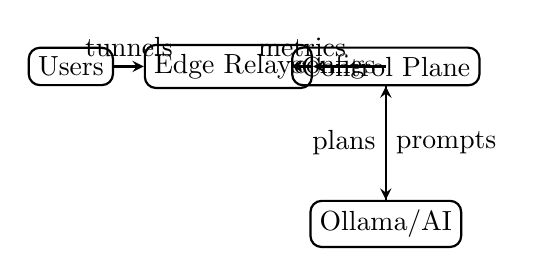
\begin{tikzpicture}[node distance=2cm,>=stealth,thick]
        \node (users) [draw, rounded corners] {Users};
        \node (edge) [draw, rounded corners, right of=users] {Edge Relays};
        \node (ctrl) [draw, rounded corners, right of=edge] {Control Plane};
        \node (ai) [draw, rounded corners, below of=ctrl] {Ollama/AI};
        \draw[->] (users) -- node[above]{tunnels} (edge);
        \draw[->] (edge) -- node[above]{metrics} (ctrl);
        \draw[->] (ctrl) -- node[right]{prompts} (ai);
        \draw[->] (ai) -- node[left]{plans} (ctrl);
        \draw[->] (ctrl) |- node[left]{configs} (edge);
    \end{tikzpicture}
    \caption{Operational layout with control plane driving edge relays.}
\end{figure}


\chapter{Development Story and Lessons Learned}

This chapter records how Smart Relay evolved and what decisions mattered. It captures the wisdom gained from building a production-ready AI-assisted proxy client with a modern GUI.

\section{Milestones}
\begin{itemize}
    \item \textbf{Scaffold}: set up Rust workspace, Axum control plane, AI client, and config store.
    \item \textbf{AI integration}: Ollama client with prompts that embed the live config snapshot.
    \item \textbf{Validation}: added HTTP error mapping and config validation to avoid unsafe applies.
    \item \textbf{GUI foundation}: Integrated \texttt{egui} for cross-platform native GUI with cyberpunk theme.
    \item \textbf{Subscription parsing}: Implemented Base64 decoding and multi-protocol parsing (VMess, VLESS, Shadowsocks, Trojan, SOCKS5).
    \item \textbf{System proxy integration}: Windows registry-based proxy configuration with Global/PAC mode support.
    \item \textbf{Endpoint management}: Connection testing, batch operations, and right-click context menus.
    \item \textbf{Internationalization}: Chinese character support with proper font configuration.
    \item \textbf{Comprehensive network diagnostics}: Multi-layer testing (DNS, TCP, routing, packet-level analysis) with detailed error categorization.
\end{itemize}

\section{Design Choices}

\subsection{Architecture}
\begin{itemize}
    \item Axum + Tokio for async control-plane tasks across platforms.
    \item Serde + TOML for human-friendly config with easy round trips.
    \item Adapter abstraction to decouple decision layer from core engines (xray, sing-box).
    \item Library crate structure: separate binaries for CLI and GUI, shared core logic.
    \item Immediate mode GUI (\texttt{egui}) for simplicity and cross-platform consistency.
\end{itemize}

\subsection{State Management}
\begin{itemize}
    \item \textbf{Config persistence}: TOML files in platform-specific config directories.
    \item \textbf{Async GUI}: Tokio runtime injected into \texttt{eframe} for async operations.
    \item \textbf{Channel-based communication}: \texttt{mpsc::channel} for passing async results to GUI thread.
    \item \textbf{One-time initialization}: Font configuration and theme application done once per frame.
\end{itemize}

\section{Critical Lessons Learned}

\subsection{Async Operations in Immediate Mode GUI}

The biggest challenge was integrating async operations (network requests, endpoint testing) with \texttt{egui}'s immediate mode update loop. \textbf{Key insight}: \texttt{eframe} runs in a synchronous context, but async operations require a Tokio runtime.

\textbf{Solution pattern}:
\begin{verbatim}
// In main.rs: Create runtime once
let rt = Arc::new(Runtime::new().expect("Failed to create Tokio runtime"));

// Pass to App
app.set_runtime(rt.clone());

// In App methods: Use rt.spawn() instead of tokio::spawn()
let (tx, rx) = mpsc::channel();
rt.spawn(async move {
    let result = async_operation().await;
    tx.send(result).unwrap();
});

// In update loop: Check for messages
if let Ok(msg) = rx.try_recv() {
    // Update UI state
}
\end{verbatim}

\textbf{Lessons}:
\begin{itemize}
    \item Never call \texttt{tokio::spawn} directly from GUI code—always use the injected runtime.
    \item Use channels (\texttt{mpsc}) to communicate between async tasks and GUI thread.
    \item Process channel messages in the \texttt{update()} method using \texttt{try\_recv()} to avoid blocking.
    \item Store receivers as \texttt{Option<mpsc::Receiver<T>>} in App state for processing across frames.
\end{itemize}

\subsection{Chinese Character Rendering}

Initial implementation showed Chinese characters as rectangles. \textbf{Root cause}: \texttt{egui}'s default fonts don't include CJK glyphs.

\textbf{Solutions tried}:
\begin{enumerate}
    \item \textbf{egui-chinese-font crate}: Automatic system font detection (works on most systems).
    \item \textbf{Manual font loading}: Fallback to Windows system fonts (\texttt{C:\textbackslash Windows\textbackslash Fonts\textbackslash msyh.ttc}).
    \item \textbf{Embedded fonts}: For maximum compatibility, embed Noto Sans CJK or similar.
\end{enumerate}

\textbf{Best practice}: Always test with actual Unicode content (subscription URLs with Chinese endpoint names) during development, not just ASCII.

\subsection{Windows System Proxy Integration}

Windows proxy configuration requires registry manipulation. \textbf{Key discovery}: Using \texttt{winreg} crate is more reliable than \texttt{netsh} commands.

\textbf{Implementation pattern}:
\begin{verbatim}
use winreg::enums::*;
use winreg::RegKey;

let hkcu = RegKey::predef(HKEY_CURRENT_USER);
let internet_settings = hkcu.open_subkey_with_flags(
    r"Software\Microsoft\Windows\CurrentVersion\Internet Settings",
    KEY_WRITE,
)?;

// Global proxy
internet_settings.set_value("ProxyEnable", &1u32)?;
internet_settings.set_value("ProxyServer", &proxy_str)?;
internet_settings.set_value("ProxyOverride", &exceptions)?;

// PAC mode
internet_settings.set_value("ProxyEnable", &0u32)?;
internet_settings.set_value("AutoConfigURL", &pac_url)?;
\end{verbatim}

\textbf{Lessons}:
\begin{itemize}
    \item Registry writes require \texttt{KEY\_WRITE} permission.
    \item Always provide user feedback when proxy changes are applied.
    \item Disable proxy on disconnect to restore user's original settings.
    \item Handle errors gracefully—proxy setup failures shouldn't crash the app.
\end{itemize}

\subsection{Subscription Parsing}

Subscription URLs return Base64-encoded content with multiple proxy protocols. \textbf{Challenges}:
\begin{itemize}
    \item Base64 decoding can fail—always handle errors.
    \item VMess JSON parsing requires handling multiple field names (\texttt{ps}, \texttt{name}, \texttt{remark}).
    \item Some protocols (VLESS, Trojan) have complex URL schemes.
    \item UTF-8 encoding must be preserved for Chinese endpoint names.
\end{itemize}

\textbf{Robust parsing pattern}:
\begin{verbatim}
// Try Base64 decode
let decoded = general_purpose::STANDARD.decode(base64_part)
    .map_err(|e| format!("Base64 decode failed: {}", e))?;

// Convert to UTF-8
let json_str = String::from_utf8(decoded)
    .map_err(|e| format!("UTF-8 decode failed: {}", e))?;

// Parse JSON with fallback field names
let name = json.get("ps")
    .or_else(|| json.get("name"))
    .or_else(|| json.get("remark"))
    .and_then(|v| v.as_str())
    .unwrap_or("Unknown Server");
\end{verbatim}

\subsection{Endpoint Testing and Connection Management}

Testing endpoints requires async TCP connections. \textbf{Pattern}:
\begin{verbatim}
pub async fn test_endpoint(host: &str, port: u16) -> Result<u64> {
    let start = Instant::now();
    match timeout(Duration::from_secs(5), 
                  TcpStream::connect((host, port))).await {
        Ok(Ok(_stream)) => Ok(start.elapsed().as_millis() as u64),
        Ok(Err(e)) => Err(anyhow!("Connection failed: {}", e)),
        Err(_) => Err(anyhow!("Connection timeout")),
    }
}
\end{verbatim}

\textbf{State management}:
\begin{itemize}
    \item Track testing state per endpoint (\texttt{testing: bool}).
    \item Store results in endpoint struct (\texttt{latency: Option<u64>}).
    \item Use visual indicators (spinner, color-coded latency).
    \item Batch testing: spawn multiple tests concurrently using \texttt{futures::join\_all}.
\end{itemize}

\subsection{Right-Click Context Menus}

\texttt{egui} doesn't have built-in context menus. \textbf{Solution}: Use \texttt{egui::Window} with fixed position.

\textbf{Pattern}:
\begin{verbatim}
// Detect right-click
if row_response.secondary_clicked() {
    self.right_click_menu = Some((
        row_response.interact_pointer_pos().unwrap(),
        idx
    ));
}

// Show menu window
if let Some((pos, idx)) = self.right_click_menu {
    egui::Window::new("context_menu")
        .fixed_pos(pos)
        .collapsible(false)
        .title_bar(false)
        .show(ui.ctx(), |ui| {
            // Menu items
        });
}
\end{verbatim}

\section{What Worked Well}
\begin{itemize}
    \item Small prompts with explicit sections lead to clearer AI responses.
    \item Early validation hooks prevented bad configs from reaching adapters.
    \item Keeping the control plane stateless (config on disk) simplifies restart/upgrade.
    \item \textbf{Channel-based async communication}: Clean separation between async tasks and GUI updates.
    \item \textbf{Default trait implementations}: Using \texttt{Default} for struct initialization reduces boilerplate.
    \item \textbf{Error handling}: Using \texttt{anyhow::Result} for error propagation simplifies debugging.
    \item \textbf{Visual feedback}: Color-coded latency, connection indicators, and status messages improve UX.
\end{itemize}

\section{Common Pitfalls and Solutions}

\subsection{Pitfall: "No reactor running" Error}
\textbf{Symptom}: \texttt{thread 'main' panicked: there is no reactor running}.\\
\textbf{Cause}: Calling \texttt{tokio::spawn} from non-async context.\\
\textbf{Solution}: Create \texttt{Runtime} in \texttt{main.rs} and pass to GUI via \texttt{Arc<Runtime>}.

\subsection{Pitfall: Moved Value Errors}
\textbf{Symptom}: \texttt{error[E0382]: use of moved value}.\\
\textbf{Cause}: Using a value in multiple async closures.\\
\textbf{Solution}: Clone values before moving into closures:
\begin{verbatim}
let host_clone = host.clone();
rt.spawn(async move {
    test_endpoint(&host_clone, port).await;
});
\end{verbatim}

\subsection{Pitfall: Font Configuration Not Applied}
\textbf{Symptom}: Chinese characters show as rectangles.\\
\textbf{Cause}: Fonts configured every frame, or default fonts don't support CJK.\\
\textbf{Solution}: Configure fonts once in \texttt{main.rs} using \texttt{egui-chinese-font}, or load system fonts manually.

\subsection{Pitfall: Grid Column Mismatch}
\textbf{Symptom}: UI layout breaks when adding new columns.\\
\textbf{Cause}: \texttt{num\_columns} doesn't match actual columns rendered.\\
\textbf{Solution}: Always update \texttt{num\_columns} when modifying grid structure.

\section{What to Improve Next}
\begin{itemize}
    \item Add schema-validated JSON outputs from AI to reduce parsing ambiguity.
    \item Implement real adapters and probe-driven scoring loops.
    \item Build integration tests for API endpoints and adapter lifecycles.
    \item Add CI to run \texttt{cargo fmt/clippy/test} and LaTeX build checks.
    \item \textbf{Test result persistence}: Store test results in config for faster UI updates.
    \item \textbf{Connection pooling}: Reuse TCP connections for batch testing.
    \item \textbf{Clipboard integration}: Copy endpoint URLs to clipboard from context menu.
    \item \textbf{Export/Import}: Save endpoint lists as JSON for backup/sharing.
\end{itemize}

\section{Performance Considerations}

\begin{itemize}
    \item \textbf{Subscription parsing}: Large subscriptions (80+ endpoints) parse in \textasciitilde{}200ms—acceptable for one-time import.
    \item \textbf{Endpoint testing}: 5-second timeout per endpoint; batch testing runs concurrently.
    \item \textbf{GUI responsiveness}: All async operations are non-blocking; UI remains interactive.
    \item \textbf{Memory}: Endpoint list stored in memory; consider pagination for 1000+ endpoints.
\end{itemize}

\subsection{Network Diagnostics and Deep Packet Analysis}

One of the most challenging aspects was implementing comprehensive endpoint testing that provides actionable diagnostics. The initial implementation only tested basic TCP connectivity, but users needed to understand \textit{why} connections failed.

\textbf{The Challenge:}
\begin{itemize}
    \item Simple TCP tests often fail even when endpoints work through proxies.
    \item Users need to understand if failures are due to DNS, routing, firewalls, or protocol issues.
    \item Different error types require different troubleshooting approaches.
\end{itemize}

\textbf{The Solution - Multi-Layer Testing:}
\begin{enumerate}
    \item \textbf{Layer 7 (DNS)}: Test hostname resolution first - if DNS fails, nothing else matters.
    \item \textbf{Layer 3 (Routing)}: Check routing table and traceroute to understand network path.
    \item \textbf{Layer 4 (TCP)}: Test TCP handshake with detailed packet flow analysis.
    \item \textbf{Layer 2/3 (Packets)}: Provide packet-level details (TCP headers, flags, sequence numbers).
    \item \textbf{Smart Testing}: Try multiple approaches (direct, via proxy, extended timeout).
\end{enumerate}

\textbf{Key Insights:}
\begin{itemize}
    \item \textbf{Connection Refused vs Timeout}: Refused means port is closed (RST received); timeout means no response (firewall dropping silently).
    \item \textbf{Packet Flow Visualization}: Showing "SYN → (no response)" helps users understand firewall behavior.
    \item \textbf{Error Categorization}: DNS failures, connection refused, timeouts, and network unreachable each require different fixes.
    \item \textbf{Diagnostic Depth}: The more detailed the diagnostics, the easier it is for users (and AI) to diagnose issues.
\end{itemize}

\textbf{Implementation Details:}
\begin{itemize}
    \item Used \texttt{tokio::net::lookup\_host} for DNS resolution with timeout.
    \item Used \texttt{tokio::net::TcpStream::connect} for TCP testing with configurable timeouts.
    \item Integrated system commands (\texttt{ipconfig}, \texttt{route}, \texttt{tracert}) for routing information.
    \item Created detailed diagnostic messages explaining packet flow and connection states.
    \item Categorized errors to provide actionable feedback (e.g., "Firewall dropping silently" vs "Port closed").
\end{itemize}

This multi-layer approach provides the context needed to understand VPN connection issues, which is especially important when endpoints may work through proxies but fail direct connections.

\section{Personal Checklist for Contributors}
\begin{itemize}
    \item Run \texttt{cargo test} before pushing changes.
    \item Keep prompts and configs under version control to aid rollbacks.
    \item Document decisions in \texttt{docs/dev\_story.md} to keep the narrative fresh.
    \item \textbf{Test with real data}: Use actual subscription URLs, not mock data.
    \item \textbf{Test on target platform}: Windows proxy features only work on Windows.
    \item \textbf{Handle errors gracefully}: Never panic on user input or network errors.
    \item \textbf{Provide feedback}: Show loading states, success messages, and error details.
    \item \textbf{Understand network layers}: When debugging connection issues, think about which OSI layer is failing.
    \item \textbf{Provide detailed diagnostics}: Users need context to understand why connections fail.
\end{itemize}


\chapter{Modern GUI Design with Cyberpunk Aesthetics}

This chapter covers the design and implementation of the Smart Relay graphical user interface, built with Rust's \texttt{egui} framework. We explore how to create a modern, AI-assisted interface that simplifies complex networking operations while maintaining a distinctive cyberpunk visual identity.

\section{Design Philosophy}

The GUI is designed with several key principles:

\begin{itemize}
    \item \textbf{Simplicity through AI}: Complex configuration is abstracted away by AI-driven recommendations
    \item \textbf{Visual Feedback}: Real-time status indicators and health monitoring
    \item \textbf{Cross-Platform}: Native performance on Windows, macOS, and Linux
    \item \textbf{Cyberpunk Aesthetic}: Dark themes with neon accents for a distinctive look
\end{itemize}

\section{Architecture Overview}

The GUI communicates with the control plane via HTTP REST API, allowing separation of concerns:

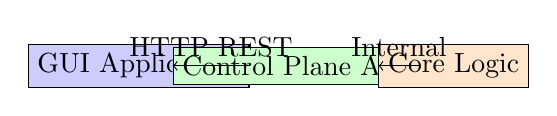
\begin{tikzpicture}[node distance=2cm, auto]
    \node[draw, rectangle, fill=blue!20] (gui) {GUI Application};
    \node[draw, rectangle, fill=green!20, right of=gui] (api) {Control Plane API};
    \node[draw, rectangle, fill=orange!20, right of=api] (core) {Core Logic};
    
    \draw[->] (gui) -- node[above] {HTTP REST} (api);
    \draw[->] (api) -- node[above] {Internal} (core);
\end{tikzpicture}

\section{egui Framework}

\texttt{egui} (immediate mode GUI) provides:

\begin{itemize}
    \item Cross-platform rendering (OpenGL via \texttt{glow} or \texttt{wgpu})
    \item Immediate mode: no retained widget state
    \item Built-in widgets: buttons, text inputs, tables, etc.
    \item Customizable theming
\end{itemize}

\section{Theme Implementation}

The cyberpunk theme uses a dark palette with neon accents and \textbf{white text for optimal contrast}:

\begin{verbatim}
Background:    #0b0f1a (dark navy)
Primary Accent: #00f0ff (cyan)
Secondary:     #ff6bd6 (pink)
Warning:       #ffc800 (amber)
Text:          WHITE (for maximum contrast on dark background)
\end{verbatim}

All text elements use white color to ensure readability against the dark background, with colored accents used only for highlights and status indicators.

\section{Key UI Components}

\subsection{Overview Tab}

The main dashboard showing:
\begin{itemize}
    \item \textbf{Current Connection}: Real-time status, latency, bandwidth usage
    \item \textbf{Quick Stats}: Total endpoints, active connections, subscription count
    \item Connection controls (connect/disconnect)
\end{itemize}

\subsection{Endpoints Tab}

Comprehensive endpoint management with advanced features:

\begin{itemize}
    \item Visual table with enable/disable toggles
    \item Endpoint details: name, host, port, protocol
    \item \textbf{Latency display}: Color-coded latency indicators
    \begin{itemize}
        \item Green: < 100ms (excellent)
        \item Yellow: 100-300ms (good)
        \item Red: > 300ms (poor)
    \end{itemize}
    \item \textbf{Connection status}: Visual highlight for connected endpoints
    \item \textbf{Actions}: Connect, Disconnect, Test, Edit, Delete
    \item \textbf{Right-click context menu}: Batch operations and quick actions
    \item Add/Edit dialog with protocol selection (VMess, VLESS, Shadowsocks, Trojan, SOCKS5)
\end{itemize}

\subsubsection{Right-Click Context Menu}

A sophisticated context menu provides quick access to common operations:

\begin{itemize}
    \item \textbf{Test Connection}: Single endpoint latency test
    \item \textbf{Test All Selected}: Batch test all enabled endpoints concurrently
    \item \textbf{Connect/Disconnect}: Quick connection toggle
    \item \textbf{Edit}: Modify endpoint configuration
    \item \textbf{Delete}: Remove endpoint (with confirmation)
    \item \textbf{Copy URL}: Copy endpoint URL to clipboard (future)
\end{itemize}

Implementation uses \texttt{egui::Window} with fixed positioning at the click location.

\subsection{Subscriptions Tab}

Subscription import and management:
\begin{itemize}
    \item Import from URL or file
    \item Subscription list with update timestamps
    \item Endpoint count per subscription
    \item Update and delete operations
\end{itemize}

\subsection{Configuration Tab}

Client and port configuration with system proxy integration:

\begin{itemize}
    \item \textbf{Port Configuration}: Local port, SOCKS5 port, HTTP port (with validation)
    \item \textbf{Client Parameters}:
    \begin{itemize}
        \item Auto Start on Boot
        \item Start Minimized
        \item Allow LAN Connections
        \item Use Local DNS
    \end{itemize}
    \item \textbf{System Proxy Mode}:
    \begin{itemize}
        \item \textbf{Unchanged}: Don't modify system proxy settings
        \item \textbf{Direct}: Disable system proxy (no proxy)
        \item \textbf{Global}: Route all traffic through proxy
        \item \textbf{PAC}: Use Proxy Auto-Configuration script
    \end{itemize}
    \item \textbf{Proxy Exceptions}: Semicolon-separated list of domains/IPs to bypass
    \item \textbf{Apply Proxy Settings}: Button to apply configuration to Windows system
\end{itemize}

When connecting to an endpoint, if "Apply to System" is enabled, the Windows system proxy is automatically configured according to the selected mode. On disconnect, the proxy is disabled to restore original settings.

\subsection{Xray Settings Tab}

Advanced Xray core configuration:
\begin{itemize}
    \item Log level (Debug, Info, Warning, Error)
    \item DNS servers configuration (multi-line)
    \item Routing domain strategy (AsIs, IPIfNonMatch, IPOnDemand)
    \item Traffic sniffing toggle
    \item Packet fragmentation toggle
\end{itemize}

\subsection{AI Assistant Tab}

AI-powered configuration assistance:
\begin{itemize}
    \item Natural language goal input
    \item AI recommendation display
    \item One-click configuration application
    \item Integration with Ollama backend
\end{itemize}

\subsection{Status Bar}

Real-time health monitoring of the control plane with visual indicators:
\begin{itemize}
    \item Cyan pulse: Online and healthy
    \item Pink: Connection error
    \item Yellow: Checking status
    \item Gray: Not connected
\end{itemize}

\section{Async State Management}

Since \texttt{egui} is immediate mode, async operations require careful handling. The critical insight is that \texttt{eframe} runs in a synchronous context, but network operations require a Tokio runtime.

\subsection{Runtime Injection Pattern}

\begin{verbatim}
// In main.rs: Create runtime once
let rt = Arc::new(Runtime::new().expect("Failed to create Tokio runtime"));

eframe::run_native("Smart Relay", options, Box::new(move |_cc| {
    let mut app = App::default();
    app.set_runtime(rt.clone());  // Inject runtime
    Box::new(app)
}));

// In App: Store runtime and use for async operations
pub struct App {
    runtime: Option<Arc<Runtime>>,
    // ... other fields
}

fn test_endpoint(&mut self, idx: usize) {
    let rt = self.runtime.as_ref().unwrap();
    let (tx, rx) = mpsc::channel();
    
    rt.spawn(async move {  // Use rt.spawn, not tokio::spawn
        let result = async_operation().await;
        tx.send(result).unwrap();
    });
    
    // Store receiver for processing in update loop
    self.test_receiver = Some(rx);
}

// In update(): Process messages
if let Some(ref mut rx) = self.test_receiver {
    if let Ok(result) = rx.try_recv() {
        // Update UI state with result
    }
}
\end{verbatim}

\subsection{Channel-Based Communication}

Use \texttt{mpsc::channel} for one-way communication from async tasks to GUI:

\begin{itemize}
    \item \textbf{Sender}: Created in async task, sends results.
    \item \textbf{Receiver}: Stored in App state, checked in \texttt{update()} loop.
    \item \textbf{Non-blocking}: Use \texttt{try\_recv()} to avoid blocking the UI thread.
    \item \textbf{Cleanup}: Remove receiver from state after processing all messages.
\end{itemize}

\section{Packaging for Multi-Platform}

\subsection{Windows}

Use PowerShell script to create release zip:
\begin{verbatim}
.\scripts\package-windows.ps1
\end{verbatim}

Creates: \texttt{smart-relay-windows-x86\_64-v0.1.0.zip}

\subsection{Linux}

Creates tarball with binaries:
\begin{verbatim}
bash scripts/package-linux.sh
\end{verbatim}

For \texttt{.deb} packages, additional tooling required (\texttt{cargo-deb}).

\subsection{macOS}

Creates \texttt{.app} bundle and optionally \texttt{.dmg}:
\begin{verbatim}
bash scripts/package-macos.sh
\end{verbatim}

\section{Font Configuration and Internationalization}

\subsection{Chinese Character Support}

Proper font configuration is essential for displaying Chinese characters in endpoint names. The implementation uses a two-tier approach:

\begin{enumerate}
    \item \textbf{Primary}: \texttt{egui-chinese-font} crate automatically detects and loads system Chinese fonts.
    \item \textbf{Fallback}: Manual loading of Windows system fonts (\texttt{msyh.ttc}, \texttt{simsun.ttc}) if automatic detection fails.
\end{enumerate}

\textbf{Key lesson}: Always test with real Unicode content during development, not just ASCII placeholder text.

\subsection{Font Loading Pattern}

\begin{verbatim}
// In main.rs: Setup fonts once during initialization
use egui_chinese_font::setup_chinese_fonts;

eframe::run_native("Smart Relay", options, Box::new(move |cc| {
    if let Err(e) = setup_chinese_fonts(&cc.egui_ctx) {
        eprintln!("Warning: Failed to load Chinese fonts: {}", e);
    }
    // ... rest of initialization
}));
\end{verbatim}

\section{Best Practices}

\begin{itemize}
    \item \textbf{Keep UI responsive}: Offload heavy work to background tasks using Tokio runtime.
    \item \textbf{Provide clear feedback}: Show loading states, success messages, and detailed error messages.
    \item \textbf{Use consistent visual language}: Colors, spacing, and typography should be consistent throughout.
    \item \textbf{Test on all target platforms}: Windows proxy features only work on Windows.
    \item \textbf{Handle errors gracefully}: Never panic on user input or network errors—show user-friendly messages.
    \item \textbf{Visual indicators}: Use color coding for status (green/yellow/red for latency, connection state).
    \item \textbf{Right-click menus}: Provide context-sensitive actions for power users.
    \item \textbf{Async operations}: Always use channels to communicate between async tasks and GUI thread.
    \item \textbf{Font configuration}: Test with actual Unicode content, not just ASCII.
    \item \textbf{State management}: Use \texttt{Default} trait for struct initialization to reduce boilerplate.
\end{itemize}

\section{Future Enhancements}

\begin{itemize}
    \item Real-time connection graphs and bandwidth visualization
    \item Advanced filtering and search with regex support
    \item Plugin system for custom widgets and protocol handlers
    \item Dark/light theme toggle (currently cyberpunk dark only)
    \item Full internationalization (i18n) with language packs
    \item Endpoint grouping and tagging for organization
    \item Connection history and statistics
    \item Export/import endpoint lists as JSON
    \item Clipboard integration for sharing endpoint URLs
    \item Keyboard shortcuts for power users
    \item Real-time latency monitoring with charts
\end{itemize}


\chapter{Xray-Core Mathematics: Cryptographic Foundations and Protocol Design}

This chapter provides a deep mathematical and algorithmic analysis of Xray-core's cryptographic implementations. We explore stream ciphers, block ciphers, key exchange protocols, and reliable transport mechanisms with detailed mathematical formulations, TikZ diagrams, and code examples from the Xray-core source code.

\section{Introduction to Xray-Core Cryptography}

Xray-core implements multiple cryptographic primitives for secure proxy communication:
\begin{itemize}
    \item \textbf{Stream Ciphers}: ChaCha20 for high-performance encryption
    \item \textbf{Block Ciphers}: AES in multiple modes (CFB, CTR, GCM)
    \item \textbf{Key Exchange}: X25519 (Curve25519) and ML-KEM-768 for post-quantum security
    \item \textbf{AEAD}: Authenticated Encryption with Associated Data for integrity
    \item \textbf{Hash Functions}: FNV-1a, MD5, SHA-3, BLAKE3
    \item \textbf{Reliable Transport}: KCP protocol with sliding window algorithms
\end{itemize}

\section{ChaCha20 Stream Cipher}

ChaCha20 is a stream cipher designed by Daniel J. Bernstein, providing high performance and security. Xray-core implements ChaCha20 for efficient encryption of proxy traffic.

\subsection{Mathematical Foundation}

ChaCha20 operates on a 512-bit state organized as 16 words of 32 bits each. The state is initialized with:
\begin{itemize}
    \item 4 constant words: $c_0 = \texttt{0x61707865}$, $c_1 = \texttt{0x3320646e}$, $c_2 = \texttt{0x79622d32}$, $c_3 = \texttt{0x6b206574}$
    \item 8 key words: $k_0, k_1, \ldots, k_7$ (256-bit key)
    \item 4 nonce/counter words: $n_0, n_1, n_2, n_3$ (128-bit nonce + counter)
\end{itemize}

The initial state matrix is:
\[
S = \begin{bmatrix}
c_0 & c_1 & c_2 & c_3 \\
k_0 & k_1 & k_2 & k_3 \\
k_4 & k_5 & k_6 & k_7 \\
n_0 & n_1 & n_2 & n_3
\end{bmatrix}
\]

\subsection{Quarter-Round Operation}

ChaCha20 uses a quarter-round function $QR(a, b, c, d)$ that operates on four 32-bit words:
\begin{align}
a &\leftarrow a + b \\
d &\leftarrow (d \oplus a) \lll 16 \\
c &\leftarrow c + d \\
b &\leftarrow (b \oplus c) \lll 12 \\
a &\leftarrow a + b \\
d &\leftarrow (d \oplus a) \lll 8 \\
c &\leftarrow c + d \\
b &\leftarrow (b \oplus c) \lll 7
\end{align}

where $\lll$ denotes left rotation and $\oplus$ is XOR.

\begin{figure}[h]
    \centering
    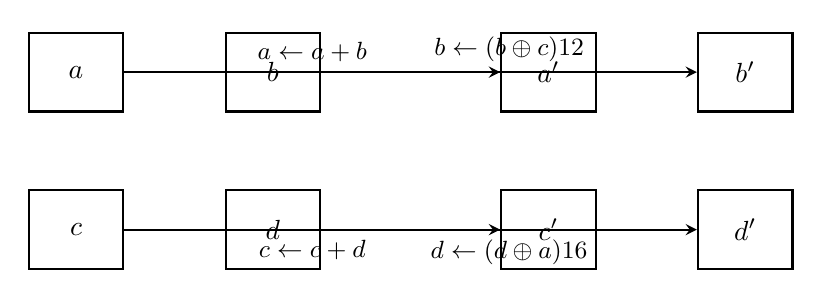
\begin{tikzpicture}[node distance=2cm,>=stealth,thick]
        \node (a1) [draw, rectangle, minimum width=1.2cm, minimum height=1cm] {$a$};
        \node (b1) [draw, rectangle, minimum width=1.2cm, minimum height=1cm, right of=a1, xshift=0.5cm] {$b$};
        \node (c1) [draw, rectangle, minimum width=1.2cm, minimum height=1cm, below of=a1] {$c$};
        \node (d1) [draw, rectangle, minimum width=1.2cm, minimum height=1cm, right of=c1, xshift=0.5cm] {$d$};
        
        \node (a2) [draw, rectangle, minimum width=1.2cm, minimum height=1cm, right of=b1, xshift=1.5cm] {$a'$};
        \node (b2) [draw, rectangle, minimum width=1.2cm, minimum height=1cm, right of=a2, xshift=0.5cm] {$b'$};
        \node (c2) [draw, rectangle, minimum width=1.2cm, minimum height=1cm, below of=a2] {$c'$};
        \node (d2) [draw, rectangle, minimum width=1.2cm, minimum height=1cm, right of=c2, xshift=0.5cm] {$d'$};
        
        \draw[->] (a1) -- node[above, font=\small] {$a \leftarrow a+b$} (a2);
        \draw[->] (b1) -- node[above, font=\small] {$b \leftarrow (b \oplus c) \lll 12$} (b2);
        \draw[->] (c1) -- node[below, font=\small] {$c \leftarrow c+d$} (c2);
        \draw[->] (d1) -- node[below, font=\small] {$d \leftarrow (d \oplus a) \lll 16$} (d2);
    \end{tikzpicture}
    \caption{ChaCha20 Quarter-Round Operation Flow}
\end{figure}

\subsection{ChaCha20 Block Function}

The ChaCha20 block function applies 20 rounds (10 double rounds) of column and diagonal mixing:

\begin{verbatim}
// From Xray-core: common/crypto/internal/chacha.go
func ChaCha20Block(state *[16]uint32, output []byte, rounds int) {
    working := *state  // Copy state
    
    // Column rounds (even rounds)
    for i := 0; i < rounds/2; i++ {
        QR(&working[0], &working[4], &working[8],  &working[12])  // Column 0
        QR(&working[1], &working[5], &working[9],  &working[13])  // Column 1
        QR(&working[2], &working[6], &working[10], &working[14])  // Column 2
        QR(&working[3], &working[7], &working[11], &working[15])  // Column 3
        
        // Diagonal rounds (odd rounds)
        QR(&working[0], &working[5], &working[10], &working[15])  // Diagonal 0
        QR(&working[1], &working[6], &working[11], &working[12])  // Diagonal 1
        QR(&working[2], &working[7], &working[8],  &working[13])  // Diagonal 2
        QR(&working[3], &working[4], &working[9],  &working[14])  // Diagonal 3
    }
    
    // Add original state (modular addition)
    for i := 0; i < 16; i++ {
        binary.LittleEndian.PutUint32(output[i*4:], working[i] + state[i])
    }
}
\end{verbatim}

The output keystream is computed as:
\[
\text{keystream} = S_{\text{initial}} + S_{\text{working}} \pmod{2^{32}}
\]

\subsection{ChaCha20 Stream Generation}

Xray-core generates a continuous keystream by incrementing the counter and generating new blocks:

\begin{verbatim}
// From Xray-core: common/crypto/internal/chacha.go
func (s *ChaCha20Stream) XORKeyStream(dst, src []byte) {
    i := 0
    max := len(src)
    for i < max {
        gap := blockSize - s.offset  // blockSize = 64 bytes
        
        limit := i + gap
        if limit > max {
            limit = max
        }
        
        // XOR with current block
        o := s.offset
        for j := i; j < limit; j++ {
            dst[j] = src[j] ^ s.block[o]
            o++
        }
        
        i += gap
        s.offset = o
        
        // Generate next block if needed
        if o == blockSize {
            s.offset = 0
            s.state[12]++  // Increment counter
            ChaCha20Block(&s.state, s.block[:], s.rounds)
        }
    }
}
\end{verbatim}

The encryption/decryption is simply:
\[
\text{ciphertext} = \text{plaintext} \oplus \text{keystream}
\]

\section{AES Encryption Modes}

Xray-core supports multiple AES modes: CFB (Cipher Feedback), CTR (Counter), and GCM (Galois/Counter Mode).

\subsection{AES-CFB (Cipher Feedback Mode)}

CFB mode turns AES into a stream cipher. The encryption process is:

\[
C_i = P_i \oplus E_K(S_i)
\]
\[
S_{i+1} = (S_i \ll 8) | C_i
\]

where $S_i$ is the shift register state, $P_i$ is plaintext, $C_i$ is ciphertext, and $E_K$ is AES encryption.

\begin{figure}[h]
    \centering
    \begin{tikzpicture}[node distance=4cm,>=stealth,thick]
        \node (iv) [draw, rectangle, minimum width=1.5cm, minimum height=1cm] {IV};
        \node (aes1) [draw, rectangle, right of=iv, minimum width=2cm, minimum height=1cm] {AES Encrypt};
        \node (xor1) [draw, circle, right of=aes1, minimum size=1cm] {$\oplus$};
        \node (c1) [draw, rectangle, right of=xor1, minimum width=1.5cm, minimum height=1cm] {$C_1$};
        \node (shift) [draw, rectangle, below of=aes1, minimum width=2cm, minimum height=1cm, yshift=-0.5cm] {Shift Register};
        \node (aes2) [draw, rectangle, right of=shift, minimum width=2cm, minimum height=1cm] {AES Encrypt};
        \node (xor2) [draw, circle, right of=aes2, minimum size=1cm] {$\oplus$};
        \node (c2) [draw, rectangle, right of=xor2, minimum width=1.5cm, minimum height=1cm] {$C_2$};
        
        \draw[->] (iv) -- (aes1);
        \draw[->] (aes1) -- node[above, font=\small] {$E_K(S_1)$} (xor1);
        \draw[->] (xor1) -- (c1);
        \draw[->] (c1) -- node[left, font=\small] {Shift} (shift);
        \draw[->] (shift) -- (aes2);
        \draw[->] (aes2) -- node[above, font=\small] {$E_K(S_2)$} (xor2);
        \draw[->] (xor2) -- (c2);
        
        \node (p1) [above of=xor1, yshift=-0.7cm] {$P_1$};
        \node (p2) [above of=xor2, yshift=-0.7cm] {$P_2$};
        \draw[->] (p1) -- (xor1);
        \draw[->] (p2) -- (xor2);
    \end{tikzpicture}
    \caption{AES-CFB Mode Encryption Flow}
\end{figure}

\subsection{AES-CTR (Counter Mode)}

CTR mode uses AES to generate a keystream from a counter:

\[
\text{keystream}_i = E_K(\text{nonce} || \text{counter}_i)
\]
\[
C_i = P_i \oplus \text{keystream}_i
\]

\begin{verbatim}
// From Xray-core: common/crypto/aes.go
func NewAesCTRStream(key []byte, iv []byte) cipher.Stream {
    return NewAesStreamMethod(key, iv, cipher.NewCTR)
}
\end{verbatim}

\subsection{AES-GCM (Galois/Counter Mode)}

GCM provides authenticated encryption. The encryption process:

\begin{enumerate}
    \item Generate keystream: $H = E_K(0^{128})$
    \item Encrypt: $C_i = P_i \oplus E_K(\text{IV} || i)$
    \item Compute authentication tag using GHASH:
    \[
    \text{Tag} = \text{GHASH}_H(\text{AAD} || C || \text{len}(AAD) || \text{len}(C))
    \]
\end{enumerate}

GHASH operates in $\text{GF}(2^{128})$:
\[
\text{GHASH}_H(X) = X_1 \cdot H \oplus X_2 \cdot H^2 \oplus \cdots \oplus X_n \cdot H^n
\]

\begin{verbatim}
// From Xray-core: common/crypto/aes.go
func NewAesGcm(key []byte) cipher.AEAD {
    block := common.Must2(aes.NewCipher(key))
    aead := common.Must2(cipher.NewGCM(block))
    return aead
}
\end{verbatim}

\section{VMess Protocol Authentication}

VMess uses time-based authentication with UUID and alterId. The authentication process involves:

\subsection{Time-Based Nonce Generation}

VMess requires system time to be synchronized within ±120 seconds of UTC. The authentication uses:

\[
\text{nonce} = \text{MD5}(\text{UUID} || \text{timestamp} || \text{alterId})
\]

where timestamp is the current UTC time in seconds.

\subsection{VMess Authentication Hash}

The authentication uses FNV-1a hash function:

\begin{verbatim}
// From Xray-core: proxy/vmess/encoding/auth.go
func Authenticate(b []byte) uint32 {
    fnv1hash := fnv.New32a()
    common.Must2(fnv1hash.Write(b))
    return fnv1hash.Sum32()
}
\end{verbatim}

FNV-1a hash algorithm:
\[
\text{hash} = \text{FNV\_OFFSET\_BASIS}
\]
\[
\text{for each byte } b: \text{hash} = (\text{hash} \oplus b) \cdot \text{FNV\_PRIME} \pmod{2^{32}}
\]

where $\text{FNV\_OFFSET\_BASIS} = 2166136261$ and $\text{FNV\_PRIME} = 16777619$.

\subsection{ChaCha20-Poly1305 Key Derivation}

VMess derives ChaCha20-Poly1305 keys using MD5:

\begin{verbatim}
// From Xray-core: proxy/vmess/encoding/auth.go
func GenerateChacha20Poly1305Key(b []byte) []byte {
    key := make([]byte, 32)
    t := md5.Sum(b)
    copy(key, t[:])           // First 16 bytes: MD5(b)
    t = md5.Sum(key[:16])
    copy(key[16:], t[:])       // Second 16 bytes: MD5(MD5(b))
    return key
}
\end{verbatim}

Mathematically:
\[
K[0:16] = \text{MD5}(b)
\]
\[
K[16:32] = \text{MD5}(K[0:16])
\]

\section{VLESS Encryption and Key Exchange}

VLESS uses advanced key exchange mechanisms including X25519 (Curve25519) and ML-KEM-768 for post-quantum security.

\subsection{Curve25519 Key Exchange}

Curve25519 is an elliptic curve over $\mathbb{F}_{2^{255}-19}$ defined by:
\[
y^2 = x^3 + 486662x^2 + x
\]

The base point $G$ has order $8\ell$ where $\ell$ is a large prime. The key exchange:

\begin{enumerate}
    \item Client generates private key: $a \in_R [0, 2^{256})$
    \item Client computes public key: $A = aG$
    \item Server has public key: $B$
    \item Shared secret: $S = aB = abG$
    \item Derived key: $K = \text{BLAKE3}(S)$
\end{enumerate}

\begin{verbatim}
// From Xray-core: proxy/vless/encryption/client.go
privateKey, _ := ecdh.X25519().GenerateKey(rand.Reader)
nfsKey, err := privateKey.ECDH(serverPublicKey)
if err != nil {
    return nil, err
}
\end{verbatim}

\subsection{ML-KEM-768 Post-Quantum Key Exchange}

ML-KEM-768 (Module-Lattice Key Encapsulation Mechanism) provides post-quantum security:

\begin{enumerate}
    \item Server generates key pair: $(sk, pk) = \text{ML-KEM-768.KeyGen}()$
    \item Client encapsulates: $(K, ct) = \text{ML-KEM-768.Encaps}(pk)$
    \item Server decapsulates: $K' = \text{ML-KEM-768.Decaps}(sk, ct)$
    \item Shared key: $K = K'$ (with high probability)
\end{enumerate}

\begin{verbatim}
// From Xray-core: proxy/vless/encryption/client.go
if k, ok := k.(*mlkem.EncapsulationKey768); ok {
    var ciphertext []byte
    nfsKey, ciphertext = k.Encapsulate()
    copy(relays, ciphertext)  // 1088 bytes
    index = 1088
}
\end{verbatim}

\subsection{VLESS United Key Derivation}

VLESS combines multiple key exchange results:

\[
\text{UnitedKey} = \text{PFSKey} || \text{NFSKey}
\]

where PFSKey is derived from ML-KEM-768 + X25519, and NFSKey is from the relay chain.

\begin{verbatim}
// From Xray-core: proxy/vless/encryption/client.go
pfsKey := make([]byte, 32+32)  // ML-KEM-768 (32) + X25519 (32)
copy(pfsKey, mlkem768Key)
copy(pfsKey[32:], x25519Key)
c.UnitedKey = append(pfsKey, nfsKey...)
\end{verbatim}

\section{KCP Protocol: Reliable Transport Mathematics}

KCP (A Fast and Reliable ARQ Protocol) implements a sliding window protocol with adaptive retransmission.

\subsection{Sliding Window Algorithm}

KCP maintains a sending window and receiving window. The sending window tracks unacknowledged segments:

\[
\text{WindowSize} = \min(\text{CongestionWindow}, \text{ReceiveWindow})
\]

\subsection{RTT Estimation}

KCP uses exponential weighted moving average (EWMA) for RTT estimation:

\[
\text{RTT} = \alpha \cdot \text{RTT}_{\text{old}} + (1-\alpha) \cdot \text{RTT}_{\text{sample}}
\]

where $\alpha$ is typically 0.7.

\subsection{Retransmission Timeout (RTO)}

RTO is calculated using RTT and RTT variance:

\[
\text{RTO} = \text{RTT} + 4 \cdot \text{RTTVar}
\]

\begin{verbatim}
// From Xray-core: transport/internet/kcp/segment.go
type DataSegment struct {
    Conv        uint16
    Option      SegmentOption
    Timestamp   uint32      // Send timestamp
    Number      uint32      // Sequence number
    SendingNext uint32     // Next expected ACK
    payload     *buf.Buffer
    timeout     uint32      // Retransmission timeout
    transmit    uint32      // Transmission count
}
\end{verbatim}

\subsection{Fast Retransmit}

KCP implements fast retransmit when duplicate ACKs are received:

\[
\text{if } \text{dupACKs} \geq 3: \text{retransmit immediately}
\]

\begin{figure}[h]
    \centering
    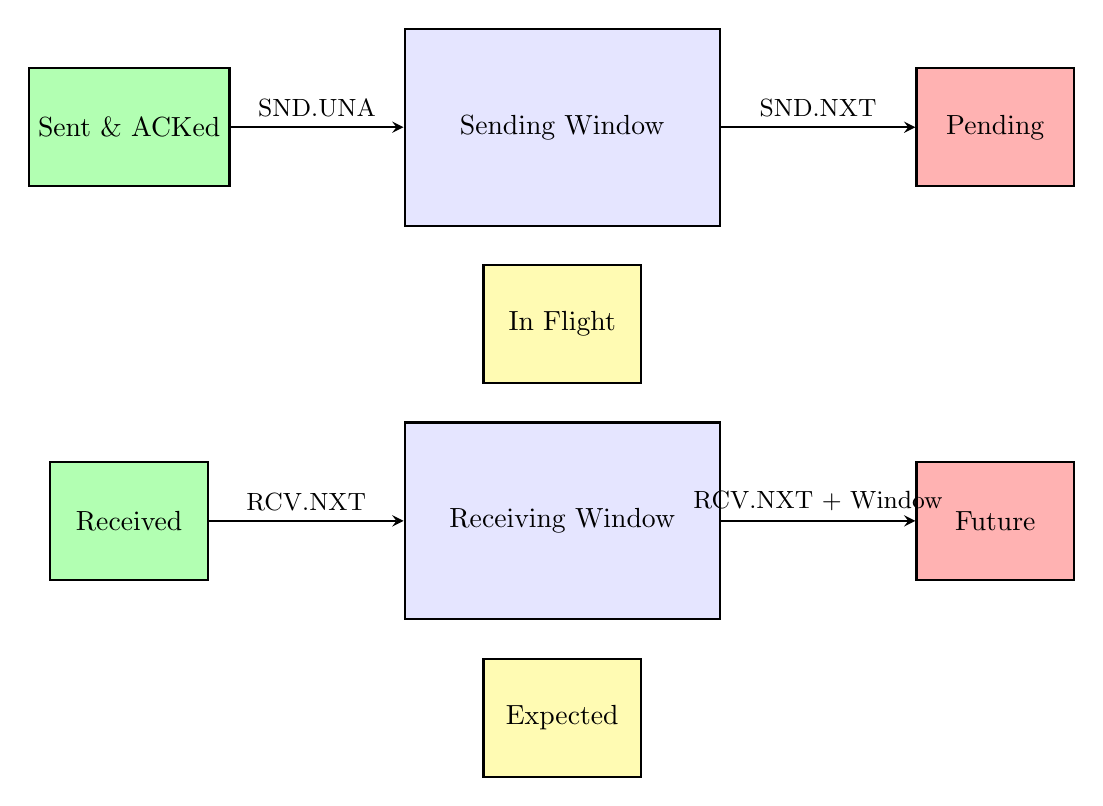
\begin{tikzpicture}[node distance=3cm,>=stealth,thick]
        \node (sw) [draw, rectangle, minimum width=4cm, minimum height=2.5cm, fill=blue!10] {Sending Window};
        \node (sent) [draw, rectangle, left of=sw, xshift=-2.5cm, fill=green!30, minimum width=2cm, minimum height=1.5cm] {Sent \& ACKed};
        \node (inflight) [draw, rectangle, fill=yellow!30, minimum width=2cm, minimum height=1.5cm, below of=sw, yshift=0.5cm] {In Flight};
        \node (pending) [draw, rectangle, right of=sw, xshift=2.5cm, fill=red!30, minimum width=2cm, minimum height=1.5cm] {Pending};
        
        \draw[->, thick] (sent) -- node[above, font=\small] {SND.UNA} (sw);
        \draw[->, thick] (sw) -- node[above, font=\small] {SND.NXT} (pending);
        
        \node (rw) [draw, rectangle, minimum width=4cm, minimum height=2.5cm, below of=sw, yshift=-2cm, fill=blue!10] {Receiving Window};
        \node (received) [draw, rectangle, left of=rw, xshift=-2.5cm, fill=green!30, minimum width=2cm, minimum height=1.5cm] {Received};
        \node (expected) [draw, rectangle, fill=yellow!30, minimum width=2cm, minimum height=1.5cm, below of=rw, yshift=0.5cm] {Expected};
        \node (future) [draw, rectangle, right of=rw, xshift=2.5cm, fill=red!30, minimum width=2cm, minimum height=1.5cm] {Future};
        
        \draw[->, thick] (received) -- node[above, font=\small] {RCV.NXT} (rw);
        \draw[->, thick] (rw) -- node[above, font=\small] {RCV.NXT + Window} (future);
    \end{tikzpicture}
    \caption{KCP Sliding Window Protocol}
\end{figure}

\section{Shadowsocks Encryption}

Shadowsocks uses stream ciphers with key derivation from password.

\subsection{Key Derivation}

Shadowsocks derives encryption keys using HKDF (HMAC-based Key Derivation Function):

\[
\text{Key} = \text{HKDF-Expand}(\text{HKDF-Extract}(\text{salt}, \text{password}), \text{info}, \text{length})
\]

\begin{verbatim}
// From Xray-core: proxy/shadowsocks/config.go
func (a *Account) getCipher() (Cipher, error) {
    switch a.CipherType {
    case CipherType_AES_128_GCM:
        return &AEADCipher{
            KeyBytes: 16,
            IVBytes:  16,
            AEAD:     createAesGcm,
        }, nil
    case CipherType_CHACHA20_POLY1305:
        return &AEADCipher{
            KeyBytes: 32,
            IVBytes:  12,
            AEAD:     createChaCha20Poly1305,
        }, nil
    }
}
\end{verbatim}

\subsection{IV Generation and Anti-Replay}

Shadowsocks uses unique IVs to prevent replay attacks:

\[
\text{IV} \in_R \{0,1\}^{128} \text{ (for AES-GCM)}
\]

The anti-replay filter checks:
\[
\text{if } \text{IV} \in \text{ReplayFilter}: \text{reject}
\]

\begin{verbatim}
// From Xray-core: proxy/shadowsocks/config.go
func (a *MemoryAccount) CheckIV(iv []byte) error {
    if a.replayFilter == nil {
        return nil
    }
    if a.replayFilter.Check(iv) {
        return nil  // IV is unique
    }
    return ErrIVNotUnique
}
\end{verbatim}

\section{AEAD: Authenticated Encryption with Associated Data}

AEAD provides both confidentiality and authenticity. Xray-core implements AEAD for multiple protocols.

\subsection{AEAD Encryption Process}

The encryption process:
\[
(C, \text{Tag}) = \text{AEAD.Seal}(\text{nonce}, \text{plaintext}, \text{AAD})
\]

where:
\begin{itemize}
    \item $C$ is the ciphertext
    \item $\text{Tag}$ is the authentication tag
    \item $\text{AAD}$ is additional authenticated data (not encrypted)
\end{itemize}

\subsection{AEAD Decryption and Verification}

The decryption process:
\[
(P, \text{valid}) = \text{AEAD.Open}(\text{nonce}, C, \text{AAD})
\]

If $\text{valid} = \text{false}$, the ciphertext is rejected.

\begin{verbatim}
// From Xray-core: common/crypto/auth.go
func (v *AEADAuthenticator) Seal(dst, plainText []byte) ([]byte, error) {
    iv := v.NonceGenerator()
    var additionalData []byte
    if v.AdditionalDataGenerator != nil {
        additionalData = v.AdditionalDataGenerator()
    }
    return v.AEAD.Seal(dst, iv, plainText, additionalData), nil
}

func (v *AEADAuthenticator) Open(dst, cipherText []byte) ([]byte, error) {
    iv := v.NonceGenerator()
    var additionalData []byte
    if v.AdditionalDataGenerator != nil {
        additionalData = v.AdditionalDataGenerator()
    }
    return v.AEAD.Open(dst, iv, cipherText, additionalData)
}
\end{verbatim}

\subsection{Nonce Generation Strategies}

Xray-core supports multiple nonce generation strategies:

\begin{enumerate}
    \item \textbf{Increasing Nonce}: Counter-based, increments for each encryption
    \[
    \text{nonce}_i = \text{nonce}_0 + i
    \]
    
    \item \textbf{Random Nonce}: Cryptographically random for each encryption
    \[
    \text{nonce}_i \in_R \{0,1\}^{96}
    \]
\end{enumerate}

\begin{verbatim}
// From Xray-core: common/crypto/auth.go
func GenerateIncreasingNonce(nonce []byte) BytesGenerator {
    c := append([]byte(nil), nonce...)
    return func() []byte {
        for i := range c {
            c[i]++
            if c[i] != 0 {
                break
            }
        }
        return c
    }
}
\end{verbatim}

\section{KCP Simple Authenticator}

KCP uses a lightweight authenticator for legacy compatibility:

\subsection{FNV Hash Authentication}

The simple authenticator uses FNV-32a hash:

\begin{verbatim}
// From Xray-core: transport/internet/kcp/crypt.go
func (a *SimpleAuthenticator) Seal(dst, nonce, plain, extra []byte) []byte {
    dst = append(dst, 0, 0, 0, 0, 0, 0)  // 4 bytes hash + 2 bytes length
    binary.BigEndian.PutUint16(dst[4:], uint16(len(plain)))
    dst = append(dst, plain...)
    
    fnvHash := fnv.New32a()
    common.Must2(fnvHash.Write(dst[4:]))  // Hash length + plaintext
    fnvHash.Sum(dst[:0])                   // Write hash to first 4 bytes
    
    // XOR obfuscation
    xtra := 4 - len(dst)%4
    if xtra != 4 {
        dst = append(dst, make([]byte, xtra)...)
    }
    xorfwd(dst)  // Forward XOR
    if xtra != 4 {
        dst = dst[:len(dst)-xtra]
    }
    return dst
}
\end{verbatim}

The authentication tag is:
\[
\text{Tag} = \text{FNV-32a}(\text{length} || \text{plaintext})
\]

\subsection{XOR Obfuscation}

KCP applies XOR obfuscation to make traffic patterns less distinguishable:

\[
\text{for } i = 0 \text{ to } n-1: \text{data}[i] = \text{data}[i] \oplus \text{data}[(i+1) \bmod n]
\]

\section{Hash Functions in Xray-Core}

Xray-core uses multiple hash functions for different purposes:

\subsection{BLAKE3}

BLAKE3 is used for key derivation in VLESS:

\[
K = \text{BLAKE3}(\text{publicKey})
\]

BLAKE3 uses a Merkle tree structure:
\[
\text{BLAKE3}(M) = \text{Compress}(\text{Chunk}_0 || \text{Chunk}_1 || \cdots || \text{Chunk}_n)
\]

\begin{verbatim}
// From Xray-core: proxy/vless/encryption/client.go
i.Hash32s[j] = blake3.Sum256(k)  // 32-byte hash of public key
\end{verbatim}

\subsection{SHA-3 (SHAKE)}

SHAKE-128 is used for size parser in VMess:

\[
\text{mask} = \text{SHAKE-128}(\text{nonce})
\]
\[
\text{encryptedSize} = \text{size} \oplus \text{mask}[0:2]
\]

\begin{verbatim}
// From Xray-core: proxy/vmess/encoding/auth.go
func NewShakeSizeParser(nonce []byte) *ShakeSizeParser {
    shake := sha3.NewShake128()
    common.Must2(shake.Write(nonce))
    return &ShakeSizeParser{shake: shake}
}

func (s *ShakeSizeParser) Encode(size uint16, b []byte) []byte {
    mask := s.next()  // Get 2 bytes from SHAKE-128 stream
    binary.BigEndian.PutUint16(b, mask^size)
    return b[:2]
}
\end{verbatim}

\section{Summary}

This chapter covered the mathematical foundations of Xray-core's cryptographic implementations:

\begin{itemize}
    \item \textbf{ChaCha20}: Stream cipher with 20-round block function and quarter-round operations
    \item \textbf{AES}: Multiple modes (CFB, CTR, GCM) for different security and performance requirements
    \item \textbf{VMess}: Time-based authentication with FNV hash and ChaCha20-Poly1305
    \item \textbf{VLESS}: Advanced key exchange with X25519 and ML-KEM-768 for post-quantum security
    \item \textbf{KCP}: Sliding window protocol with adaptive RTT estimation and fast retransmit
    \item \textbf{Shadowsocks}: HKDF-based key derivation with AEAD encryption
    \item \textbf{AEAD}: Authenticated encryption providing confidentiality and integrity
    \item \textbf{Hash Functions}: BLAKE3, SHA-3, FNV-1a for various cryptographic purposes
\end{itemize}

Understanding these mathematical foundations is essential for:
\begin{itemize}
    \item Debugging cryptographic issues
    \item Optimizing performance
    \item Implementing protocol extensions
    \item Ensuring security properties
\end{itemize}

\section{Further Reading}

\begin{itemize}
    \item ChaCha20 and Poly1305: \url{https://tools.ietf.org/html/rfc8439}
    \item AES-GCM: \url{https://nvlpubs.nist.gov/nistpubs/Legacy/SP/nistspecialpublication800-38d.pdf}
    \item Curve25519: \url{https://cr.yp.to/ecdh.html}
    \item ML-KEM: \url{https://csrc.nist.gov/publications/detail/fips/203/final}
    \item KCP Protocol: \url{https://github.com/skywind3000/kcp}
    \item BLAKE3: \url{https://github.com/BLAKE3-team/BLAKE3}
\end{itemize}


\chapter{Xray Architecture and Integration with Smart Relay}

This chapter provides a comprehensive analysis of Xray-core's internal architecture, how it processes connections, and how the Smart Relay Rust client integrates with it. We cover the complete lifecycle from configuration generation to connection routing, with detailed diagrams and code examples.

\section{Xray-Core Architecture Overview}

Xray-core is built on a modular, feature-based architecture where components are registered as \textbf{Features} and managed through dependency injection. The core instance orchestrates all features and handles their lifecycle.

\subsection{Core Components}

Xray's architecture consists of several key components:

\begin{itemize}
    \item \textbf{Instance}: The main Xray server instance that manages all features
    \item \textbf{Features}: Modular components (DNS, Routing, Inbound/Outbound Managers, etc.)
    \item \textbf{Inbound Handlers}: Accept connections from clients (SOCKS5, HTTP proxy)
    \item \textbf{Outbound Handlers}: Establish connections to VPN servers (VMess, VLESS, Shadowsocks)
    \item \textbf{Dispatcher}: Routes traffic between inbounds and outbounds
    \item \textbf{Router}: Makes routing decisions based on rules
    \item \textbf{DNS Client}: Resolves domain names
\end{itemize}

\begin{figure}[h]
    \centering
    \begin{tikzpicture}[node distance=3cm,>=stealth,thick]
        \node (instance) [draw, rectangle, minimum width=3cm, minimum height=2cm, fill=blue!20] {Xray Instance};
        
        \node (inbound) [draw, rectangle, minimum width=2.5cm, minimum height=1.5cm, left of=instance, xshift=-2cm, fill=green!20] {Inbound Manager};
        \node (outbound) [draw, rectangle, minimum width=2.5cm, minimum height=1.5cm, right of=instance, xshift=2cm, fill=red!20] {Outbound Manager};
        \node (dns) [draw, rectangle, minimum width=2.5cm, minimum height=1.5cm, below of=instance, yshift=-1cm, fill=purple!20] {DNS Client};
        \node (dispatcher) [draw, rectangle, minimum width=2.5cm, minimum height=1.5cm, above of=router, yshift=0.5cm, fill=orange!20] {Dispatcher};
        \node (router) [draw, rectangle, minimum width=2.5cm, minimum height=1.5cm, left of=dispatcher, xshift=-2cm, fill=yellow!20] {Router};

        \draw[<->] (instance) -- (inbound);
        \draw[<->] (instance) -- (outbound);
        \draw[<->] (instance) -- (router);
        \draw[<->] (instance) -- (dns);
        \draw[<->] (instance) -- (dispatcher);
        \draw[->] (dispatcher) -- (router);
        \draw[->] (router) -- (outbound);
        \draw[->] (inbound) -- (dispatcher);
    \end{tikzpicture}
    \caption{Xray-Core Architecture: Feature-Based Modular Design}
\end{figure}

\subsection{Instance Initialization}

The Xray Instance is created from a configuration object. During initialization:

\begin{enumerate}
    \item \textbf{Feature Registration}: All features (DNS, Router, Inbound/Outbound Managers) are registered
    \item \textbf{Dependency Resolution}: Features with dependencies wait until dependencies are available
    \item \textbf{Handler Creation}: Inbound and outbound handlers are created from configuration
    \item \textbf{System Initialization}: DNS client and system dialer are initialized
\end{enumerate}

\begin{verbatim}
// From Xray-core: core/xray.go
func New(config *Config) (*Instance, error) {
    server := &Instance{ctx: context.Background()}
    
    // Register all features from config
    for _, appSettings := range config.App {
        settings, err := appSettings.GetInstance()
        if err != nil {
            return nil, err
        }
        obj, err := CreateObject(server, settings)
        if err != nil {
            return nil, err
        }
        if feature, ok := obj.(features.Feature); ok {
            if err := server.AddFeature(feature); err != nil {
                return nil, err
            }
        }
    }
    
    // Add essential features if not present
    essentialFeatures := []struct {
        Type     interface{}
        Instance features.Feature
    }{
        {dns.ClientType(), localdns.New()},
        {policy.ManagerType(), policy.DefaultManager{}},
        {routing.RouterType(), routing.DefaultRouter{}},
        {stats.ManagerType(), stats.NoopManager{}},
    }
    
    // Initialize inbounds and outbounds
    if err := addInboundHandlers(server, config.Inbound); err != nil {
        return nil, err
    }
    
    if err := addOutboundHandlers(server, config.Outbound); err != nil {
        return nil, err
    }
    
    return server, nil
}
\end{verbatim}

\section{Smart Relay Rust Client Integration}

The Smart Relay Rust client manages Xray as an external process, communicating through configuration files and monitoring the process lifecycle.

\subsection{XrayAdapter Structure}

The \texttt{XrayAdapter} struct manages the Xray process and configuration:

\begin{verbatim}
// From Smart Relay: src/proxy/xray_adapter.rs
pub struct XrayAdapter {
    xray_path: PathBuf,              // Path to xray.exe binary
    process: Arc<Mutex<Option<Child>>>,  // Xray process handle
    config_path: PathBuf,            // Path to config JSON file
    socks_port: u16,                  // Configured SOCKS5 port
    http_port: u16,                   // Configured HTTP proxy port
    api_port: u16,                    // API port (for future use)
    actual_socks_port: Arc<Mutex<Option<u16>>>,  // Actual port (after fallback)
    actual_http_port: Arc<Mutex<Option<u16>>>,  // Actual port (after fallback)
}
\end{verbatim}

\subsection{Configuration Generation Flow}

The Rust client generates Xray configuration from endpoint data:

\begin{figure}[h]
    \centering
    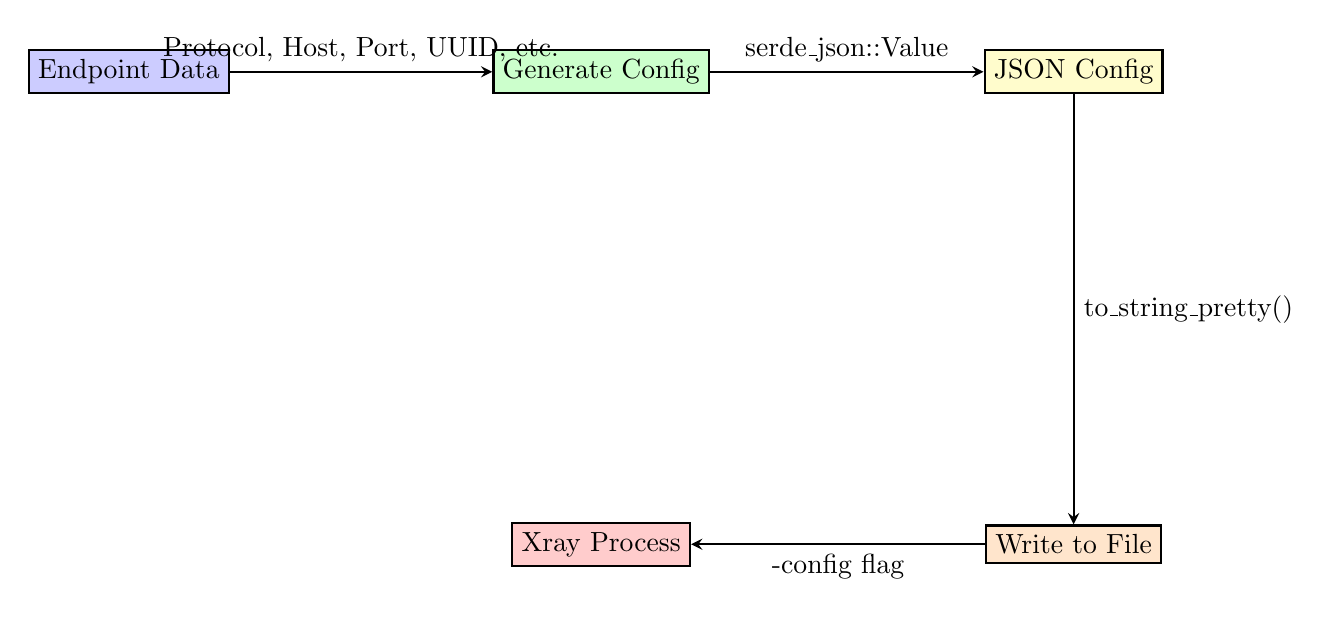
\begin{tikzpicture}[node distance=6cm,>=stealth,thick]
        \node (endpoint) [draw, rectangle, fill=blue!20] {Endpoint Data};
        \node (config) [draw, rectangle, right of=endpoint, fill=green!20] {Generate Config};
        \node (json) [draw, rectangle, right of=config, fill=yellow!20] {JSON Config};
        \node (file) [draw, rectangle, below of=json, fill=orange!20] {Write to File};
        \node (xray) [draw, rectangle, left of=file, fill=red!20] {Xray Process};
        
        \draw[->] (endpoint) -- node[above] {Protocol, Host, Port, UUID, etc.} (config);
        \draw[->] (config) -- node[above] {serde\_json::Value} (json);
        \draw[->] (json) -- node[right] {to\_string\_pretty()} (file);
        \draw[->] (file) -- node[below] {-config flag} (xray);
    \end{tikzpicture}
    \caption{Configuration Generation and Passing to Xray}
\end{figure}

\subsubsection{Configuration Generation Code}

\begin{verbatim}
// From Smart Relay: src/proxy/xray_adapter.rs
pub fn generate_config(&self, endpoint: &EndpointConfig) -> Result<Value> {
    // Generate outbound based on protocol
    let mut outbound = match endpoint.protocol.to_lowercase().as_str() {
        "vmess" => self.generate_vmess_outbound(endpoint)?,
        "vless" => self.generate_vless_outbound(endpoint)?,
        "shadowsocks" => self.generate_shadowsocks_outbound(endpoint)?,
        "trojan" => self.generate_trojan_outbound(endpoint)?,
        "socks5" => self.generate_socks5_outbound(endpoint)?,
        _ => return Err(anyhow::anyhow!("Unsupported protocol")),
    };
    
    outbound["tag"] = json!("proxy");
    
    // Build complete configuration
    let config = json!({
        "log": { "loglevel": "warning" },
        "inbounds": [
            {
                "port": socks_port,
                "protocol": "socks",
                "settings": { "auth": "noauth", "udp": true },
                "sniffing": { "enabled": true, "destOverride": ["http", "tls"] }
            },
            {
                "port": http_port,
                "protocol": "http",
                "settings": { "allowTransparent": false }
            }
        ],
        "outbounds": [
            outbound,
            { "protocol": "freedom", "tag": "direct" },
            { "protocol": "blackhole", "tag": "blocked" }
        ],
        "routing": {
            "domainStrategy": "IPOnDemand",
            "rules": [
                {
                    "type": "field",
                    "network": "tcp,udp",
                    "outboundTag": "proxy"
                }
            ]
        }
    });
    
    Ok(config)
}
\end{verbatim}

\subsection{Process Lifecycle Management}

\subsubsection{Starting Xray}

The Rust client starts Xray with careful port management and error handling:

\begin{verbatim}
// From Smart Relay: src/proxy/xray_adapter.rs
pub fn start(&self) -> Result<()> {
    let mut process_guard = self.process.lock().unwrap();
    
    if process_guard.is_some() {
        warn!("Xray is already running");
        return Ok(());
    }
    
    // Check port availability with retries
    let max_retries = 5;
    for attempt in 0..max_retries {
        let (socks_avail, http_avail) = check_ports_available_sync(
            self.socks_port, 
            self.http_port
        );
        
        if socks_avail && http_avail {
            break;
        }
        
        if attempt < max_retries - 1 {
            // Try to kill processes using ports
            let _ = self.kill_processes_using_ports();
            std::thread::sleep(Duration::from_millis(500 * (attempt + 1)));
        } else {
            // Find alternative ports
            let (alt_socks, alt_http) = find_available_ports_sync()?;
            // Update config with alternative ports
            // ...
        }
    }
    
    // Spawn Xray process
    let child = Command::new(&self.xray_path)
        .arg("-config")
        .arg(&self.config_path)
        .stdout(Stdio::piped())
        .stderr(Stdio::piped())
        .spawn()
        .context("Failed to start xray process")?;
    
    let pid = child.id();
    *process_guard = Some(child);
    
    // Wait for initialization
    std::thread::sleep(Duration::from_millis(1000));
    
    // Check if process exited immediately (port binding error)
    // If so, retry with alternative ports
    
    Ok(())
}
\end{verbatim}

\subsubsection{Stopping Xray}

\begin{verbatim}
// From Smart Relay: src/proxy/xray_adapter.rs
pub fn stop(&self) -> Result<()> {
    let mut process_guard = self.process.lock().unwrap();
    
    if let Some(mut child) = process_guard.take() {
        let pid = child.id();
        
        // On Windows, kill process tree
        #[cfg(windows)]
        {
            let _ = Command::new("taskkill")
                .args(&["/F", "/T", "/PID", &pid.to_string()])
                .output();
            let _ = child.kill();
        }
        
        // Wait for process to exit with timeout
        let start = std::time::Instant::now();
        loop {
            match child.try_wait() {
                Ok(Some(_)) => break,
                Ok(None) => {
                    if start.elapsed().as_secs() > 5 {
                        let _ = child.kill();
                        let _ = child.wait();
                        break;
                    }
                    std::thread::sleep(Duration::from_millis(100));
                }
                Err(e) => {
                    warn!("Error waiting for Xray: {}", e);
                    break;
                }
            }
        }
        
        // Wait for ports to be released
        // ...
    }
    
    Ok(())
}
\end{verbatim}

\section{Connection Flow: Client to VPN Server}

Understanding how connections flow through Xray is crucial for debugging and optimization.

\subsection{Complete Connection Path}

\begin{figure}[h]
    \centering
    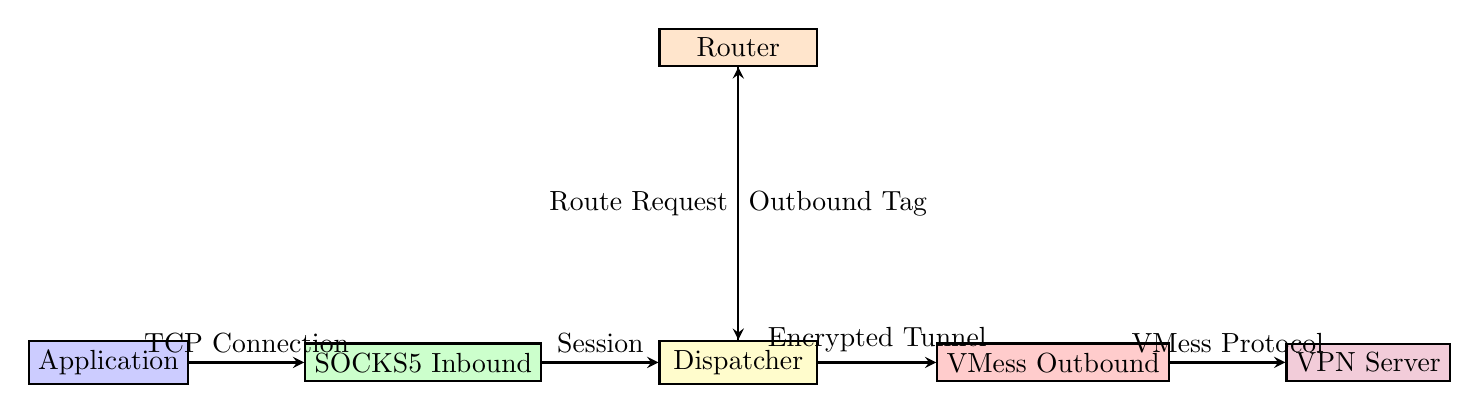
\begin{tikzpicture}[node distance=4cm,>=stealth,thick]
        \node (app) [draw, rectangle, fill=blue!20, minimum width=2cm] {Application};
        \node (socks) [draw, rectangle, right of=app, fill=green!20, minimum width=2cm] {SOCKS5 Inbound};
        \node (dispatcher) [draw, rectangle, right of=socks, fill=yellow!20, minimum width=2cm] {Dispatcher};
        \node (router) [draw, rectangle, above of=dispatcher, fill=orange!20, minimum width=2cm] {Router};
        \node (outbound) [draw, rectangle, right of=dispatcher, fill=red!20, minimum width=2cm] {VMess Outbound};
        \node (server) [draw, rectangle, right of=outbound, fill=purple!20, minimum width=2cm] {VPN Server};
        
        \draw[->] (app) -- node[above] {TCP Connection} (socks);
        \draw[->] (socks) -- node[above] {Session} (dispatcher);
        \draw[->] (dispatcher) -- node[left] {Route Request} (router);
        \draw[->] (router) -- node[right] {Outbound Tag} (dispatcher);
        \draw[->] (dispatcher) -- node[above] {Encrypted Tunnel} (outbound);
        \draw[->] (outbound) -- node[above] {VMess Protocol} (server);
    \end{tikzpicture}
    \caption{Complete Connection Flow Through Xray}
\end{figure}

\subsection{Step-by-Step Connection Processing}

\subsubsection{Step 1: Inbound Handler Accepts Connection}

When a client connects to the SOCKS5 port (e.g., 127.0.0.1:1080):

\begin{verbatim}
// Xray inbound handler accepts connection
// From Xray-core: app/proxyman/inbound/inbound.go
func (m *Manager) AddHandler(ctx context.Context, handler inbound.Handler) error {
    // Handler starts listening on configured port
    if m.running {
        return handler.Start()  // Begin accepting connections
    }
    return nil
}
\end{verbatim}

The SOCKS5 handler:
\begin{enumerate}
    \item Accepts TCP connection on port 1080
    \item Performs SOCKS5 handshake (authentication, command, address)
    \item Creates a \textbf{Session} object with destination information
    \item Passes session to the Dispatcher
\end{enumerate}

\subsubsection{Step 2: Dispatcher Receives Session}

The Dispatcher is the central routing component:

\begin{verbatim}
// From Xray-core: app/dispatcher/dispatcher.go
// The dispatcher receives a session and:
// 1. Extracts destination (IP/port or domain)
// 2. Calls Router to determine outbound
// 3. Forwards session to appropriate outbound handler
\end{verbatim}

\subsubsection{Step 3: Router Makes Routing Decision}

The Router evaluates rules to determine which outbound to use:

\begin{verbatim}
// From Xray-core: app/router/router.go
func (r *Router) PickRoute(ctx routing.Context) (routing.Route, error) {
    // Evaluate rules in order
    for _, rule := range r.rules {
        if rule.Condition.Apply(ctx) {
            // Rule matches, return associated outbound tag
            return &Route{
                outboundTag: rule.Tag,
                ruleTag: rule.RuleTag,
            }, nil
        }
    }
    
    // Default: use first outbound or direct
    return defaultRoute, nil
}
\end{verbatim}

Routing rules can match on:
\begin{itemize}
    \item \textbf{Domain}: Specific domains or patterns (e.g., \texttt{geosite:google})
    \item \textbf{IP Address}: IP ranges or GeoIP (e.g., \texttt{geoip:private})
    \item \textbf{Port}: Specific ports or ranges
    \item \textbf{Network}: TCP, UDP, or both
    \item \textbf{Source}: Source IP or tag
\end{itemize}

\subsubsection{Step 4: Outbound Handler Establishes Connection}

Once the router determines the outbound (e.g., \texttt{tag: "proxy"}), the dispatcher forwards the session to the VMess outbound handler:

\begin{verbatim}
// From Xray-core: proxy/vmess/outbound/outbound.go
// The VMess outbound handler:
// 1. Extracts destination from session
// 2. Performs VMess handshake with server:
//    - Generates authentication header (UUID, timestamp, alterId)
//    - Encrypts with ChaCha20-Poly1305 or AES-128-GCM
//    - Sends request header
// 3. Establishes encrypted tunnel
// 4. Forwards application data through tunnel
\end{verbatim}

\subsection{VMess Handshake Details}

The VMess protocol handshake involves several cryptographic operations:

\begin{enumerate}
    \item \textbf{Authentication Header Generation}:
    \[
    \text{Header} = \text{Encrypt}(\text{UUID} || \text{Timestamp} || \text{Nonce}, K)
    \]
    where $K$ is derived from the UUID and server key.
    
    \item \textbf{Request Header}:
    \begin{itemize}
        \item Version (1 byte)
        \item IV (16 bytes, random)
        \item Key (16 bytes, encrypted with server public key)
        \item V (1 byte, response authentication)
        \item Option (1 byte)
        \item Padding (variable)
        \item Command (1 byte: TCP, UDP, Mux)
        \item Port (2 bytes, big-endian)
        \item Address Type (1 byte) + Address (variable)
        \item Random bytes (variable, for padding)
    \end{itemize}
    
    \item \textbf{Response Header}:
    \begin{itemize}
        \item Response (1 byte)
        \item Option (1 byte)
        \item Command (1 byte)
        \item Port (2 bytes)
        \item Address Type + Address
    \end{itemize}
    
    \item \textbf{Data Transmission}:
    After handshake, all data is encrypted using the negotiated key and IV.
\end{enumerate}

\section{Xray Internal Data Structures}

\subsection{Session Object}

The Session object carries connection metadata through Xray:

\begin{verbatim}
// From Xray-core: common/session/session.go
type Session struct {
    ID          ID              // Unique session identifier
    User        *protocol.User  // User associated with connection
    Content     *Content        // Request content (destination, etc.)
    Inbound     *Inbound        // Inbound handler info
    Outbound    *Outbound       // Outbound handler info
    Time        time.Time       // Connection time
}
\end{verbatim}

\subsection{Content Object}

The Content object contains destination information:

\begin{verbatim}
type Content struct {
    Protocol    string          // Protocol (HTTP, TLS, etc.)
    SniffedProtocol string     // Sniffed protocol
    Domain      string          // Destination domain
    Attributes  map[string]string  // Additional attributes
}
\end{verbatim}

\section{Integration Points: Rust Client and Xray}

\subsection{Configuration File Communication}

The Rust client and Xray communicate exclusively through a JSON configuration file:

\begin{enumerate}
    \item \textbf{Rust Client}: Generates JSON config from endpoint data
    \item \textbf{File System}: Writes config to \texttt{xray\_config.json}
    \item \textbf{Xray Process}: Reads config on startup via \texttt{-config} flag
    \item \textbf{No Runtime Communication}: Xray does not accept runtime config changes (must restart)
\end{enumerate}

\begin{figure}[h]
    \centering
    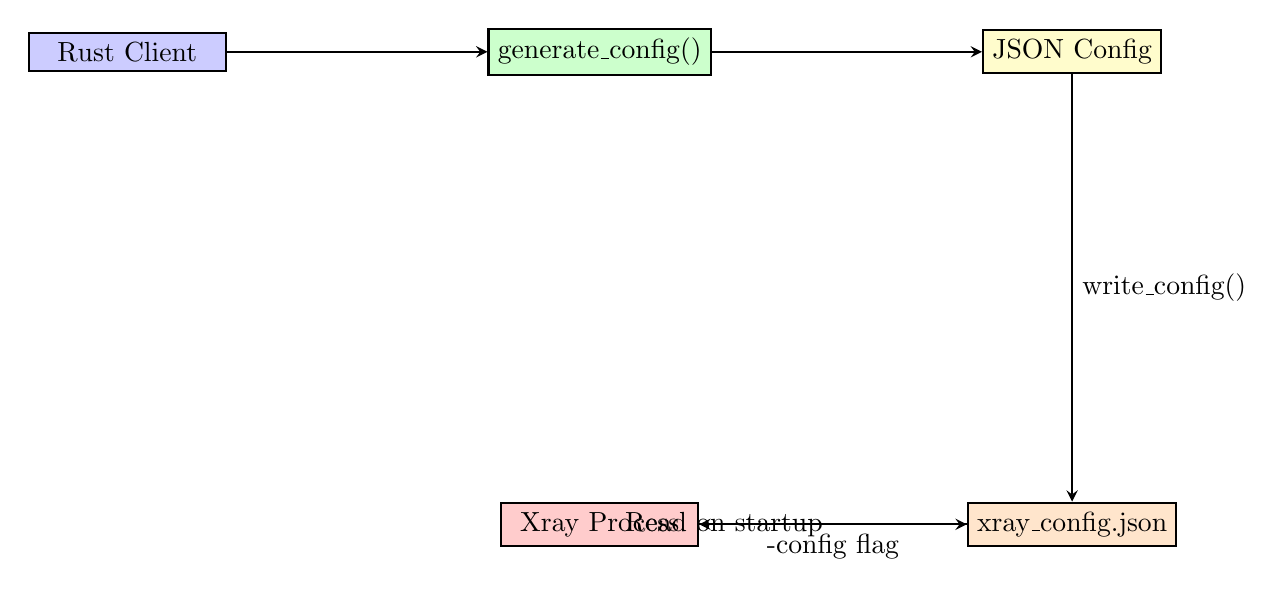
\begin{tikzpicture}[node distance=6cm,>=stealth,thick]
        \node (rust) [draw, rectangle, fill=blue!20, minimum width=2.5cm] {Rust Client};
        \node (gen) [draw, rectangle, right of=rust, fill=green!20, minimum width=2cm] {generate\_config()};
        \node (json) [draw, rectangle, right of=gen, fill=yellow!20, minimum width=2cm] {JSON Config};
        \node (file) [draw, rectangle, below of=json, fill=orange!20, minimum width=2cm] {xray\_config.json};
        \node (xray) [draw, rectangle, left of=file, fill=red!20, minimum width=2.5cm] {Xray Process};
        
        \draw[->] (rust) -- (gen);
        \draw[->] (gen) -- (json);
        \draw[->] (json) -- node[right] {write\_config()} (file);
        \draw[->] (file) -- node[below] {-config flag} (xray);
        \draw[->, dashed] (xray) -- node[left] {Read on startup} (file);
    \end{tikzpicture}
    \caption{Configuration Communication: File-Based}
\end{figure}

\subsection{Process Monitoring}

The Rust client monitors Xray's process status:

\begin{verbatim}
// From Smart Relay: src/proxy/xray_adapter.rs
pub fn is_running(&self) -> bool {
    let process_guard = self.process.lock().unwrap();
    if let Some(ref child) = *process_guard {
        match child.try_wait() {
            Ok(None) => true,   // Process still running
            Ok(Some(_)) => false,  // Process exited
            Err(_) => false,
        }
    } else {
        false
    }
}
\end{verbatim}

\subsection{Port Management}

The Rust client manages ports carefully to avoid conflicts:

\begin{enumerate}
    \item \textbf{Pre-Start Check}: Verifies ports are available before starting Xray
    \item \textbf{Retry Logic}: Retries with delays to handle TIME\_WAIT states
    \item \textbf{Process Killing}: Kills processes using ports if needed (Windows: PowerShell/taskkill)
    \item \textbf{Port Fallback}: Finds alternative ports if configured ports are unavailable
    \item \textbf{Post-Stop Verification}: Waits for ports to be released after stopping Xray
\end{enumerate}

\section{Connection Routing in Detail}

\subsection{Domain Strategy}

Xray supports multiple domain resolution strategies:

\begin{itemize}
    \item \textbf{AsIs}: Use domain as-is, resolve when needed
    \item \textbf{UseIP}: Resolve domain to IP before routing
    \item \textbf{UseIPv4}: Prefer IPv4, fallback to IPv6
    \item \textbf{UseIPv6}: Prefer IPv6, fallback to IPv4
    \item \textbf{IPIfNonMatch}: Resolve to IP if no domain rule matches
    \item \textbf{IPOnDemand}: Resolve on demand (used by Smart Relay)
\end{itemize}

\subsection{Routing Rule Evaluation}

Rules are evaluated in order until a match is found:

\begin{verbatim}
// Example routing configuration from Smart Relay
{
    "routing": {
        "domainStrategy": "IPOnDemand",
        "rules": [
            {
                "type": "field",
                "ip": ["geoip:private"],
                "outboundTag": "direct"
            },
            {
                "type": "field",
                "domain": ["geosite:ads"],
                "outboundTag": "blocked"
            },
            {
                "type": "field",
                "network": "tcp,udp",
                "outboundTag": "proxy"
            }
        ]
    }
}
\end{verbatim}

Evaluation order:
\begin{enumerate}
    \item Check IP rules (geoip:private) → route to "direct" if match
    \item Check domain rules (geosite:ads) → route to "blocked" if match
    \item Check network rules (tcp,udp) → route to "proxy" (catch-all)
\end{enumerate}

\section{Error Handling and Recovery}

\subsection{Port Binding Errors}

When Xray fails to bind to a port:

\begin{enumerate}
    \item \textbf{Detection}: Process exits immediately after spawn
    \item \textbf{Error Reading}: Read stderr to get error message
    \item \textbf{Port Fallback}: Find alternative ports
    \item \textbf{Config Update}: Update JSON config with new ports
    \item \textbf{Retry}: Spawn Xray again with new ports
\end{enumerate}

\begin{verbatim}
// From Smart Relay: src/proxy/xray_adapter.rs
if process_exited {
    // Read error output
    let error_output = read_xray_output(&mut process_guard_check)?;
    
    if error_output.contains("bind:") || error_output.contains("address already in use") {
        // Port binding error, find alternatives
        let (alt_socks, alt_http) = find_available_ports_sync()?;
        // Update config and retry
    }
}
\end{verbatim}

\subsection{Connection Failures}

When connections fail:

\begin{enumerate}
    \item \textbf{Local Proxy Check}: Verify SOCKS5/HTTP ports are listening
    \item \textbf{DNS Resolution}: Check if destination domain resolves
    \item \textbf{Direct Connection Test}: Test TCP connection to VPN server
    \item \textbf{Routing Check}: Verify routing rules are correct
    \item \textbf{Protocol Errors}: Check VMess/VLESS configuration (UUID, time sync, etc.)
\end{enumerate}

\section{Performance Considerations}

\subsection{Connection Pooling}

Xray maintains connection pools for outbound handlers to reuse connections:

\begin{itemize}
    \item \textbf{VMess}: Reuses connections when possible (same server, same user)
    \item \textbf{VLESS}: Connection reuse with session tickets
    \item \textbf{Shadowsocks}: Simple connection reuse
\end{itemize}

\subsection{Memory Management}

Xray uses buffer pools to reduce allocations:

\begin{verbatim}
// From Xray-core: common/buf/buf.go
// Buffers are pooled and reused to reduce GC pressure
type Buffer struct {
    v []byte
    // ...
}
\end{verbatim}

\subsection{Concurrency}

Xray handles connections concurrently:
\begin{itemize}
    \item Each inbound connection is handled in a separate goroutine
    \item Outbound connections are established asynchronously
    \item Routing decisions are made without blocking
\end{itemize}

\section{Summary}

This chapter covered:

\begin{itemize}
    \item \textbf{Xray Architecture}: Feature-based modular design with Instance, Features, Managers
    \item \textbf{Rust Client Integration}: XrayAdapter manages process lifecycle and configuration
    \item \textbf{Configuration Flow}: JSON config generation → file write → Xray startup
    \item \textbf{Connection Flow}: Application → Inbound → Dispatcher → Router → Outbound → VPN Server
    \item \textbf{Routing}: Rule-based routing with domain/IP/network matching
    \item \textbf{Error Handling}: Port management, connection failures, recovery strategies
    \item \textbf{Performance}: Connection pooling, buffer management, concurrency
\end{itemize}

Understanding this architecture is essential for:
\begin{itemize}
    \item Debugging connection issues
    \item Optimizing performance
    \item Implementing new features
    \item Integrating with other systems
\end{itemize}


\chapter{VMESS, VLESS, and Trojan Protocols: Deep Dive}

This chapter provides comprehensive coverage of the three major proxy protocols implemented in Xray-core: VMESS, VLESS, and Trojan. We examine their design principles, authentication mechanisms, encryption schemes, packet structures, and implementation details with mathematical formulations and code examples.

\section{VMESS Protocol}

VMESS (Versatile Message Stream) is a custom protocol designed for high-performance proxy communication with strong security guarantees. It uses time-based authentication and supports multiple encryption methods.

\subsection{Protocol Overview}

VMESS is a stateful protocol that requires:
\begin{itemize}
    \item \textbf{UUID}: 16-byte unique identifier for authentication
    \item \textbf{Time Synchronization}: System time must be within ±120 seconds of UTC
    \item \textbf{alterId}: Legacy compatibility parameter (deprecated in newer versions)
    \item \textbf{Security Type}: Encryption method (AES-128-GCM, ChaCha20-Poly1305, None, Auto)
\end{itemize}

\subsection{VMESS Handshake Process}

The VMESS handshake consists of two phases: request header and response header.

\subsubsection{Request Header Structure}

The request header contains authentication and routing information:

\begin{verbatim}
// From Xray-core: proxy/vmess/encoding/client.go
type RequestHeader struct {
    Version  byte              // Protocol version (1)
    IV       [16]byte          // Random initialization vector
    Key      [16]byte          // Random encryption key
    V        byte              // Response authentication byte
    Option   byte              // Protocol options
    Padding  byte              // Padding length
    Security SecurityType      // Encryption method
    Command  RequestCommand    // TCP, UDP, or Mux
    Address  net.Address       // Destination address
    Port     net.Port          // Destination port
}
\end{verbatim}

\subsubsection{Request Header Generation}

\begin{verbatim}
// From Xray-core: proxy/vmess/encoding/client.go
func (c *ClientSession) EncodeRequestHeader(header *protocol.RequestHeader, writer io.Writer) error {
    buffer := buf.New()
    
    // Generate random bytes for IV, Key, and V
    randomBytes := make([]byte, 33) // 16 + 16 + 1
    rand.Read(randomBytes)
    requestBodyIV := randomBytes[:16]
    requestBodyKey := randomBytes[16:32]
    responseHeader := randomBytes[32]
    
    // Write header components
    buffer.WriteByte(Version)              // Version = 1
    buffer.Write(requestBodyIV[:])        // 16 bytes IV
    buffer.Write(requestBodyKey[:])        // 16 bytes Key
    buffer.WriteByte(responseHeader)       // Response auth byte
    buffer.WriteByte(byte(header.Option))  // Options
    
    // Security and padding
    paddingLen := dice.Roll(16)  // Random padding 0-15
    security := byte(paddingLen<<4) | byte(header.Security)
    buffer.Write([]byte{security, 0, byte(header.Command)})
    
    // Destination address and port
    if header.Command != protocol.RequestCommandMux {
        addrParser.WriteAddressPort(buffer, header.Address, header.Port)
    }
    
    // Padding
    if paddingLen > 0 {
        buffer.ReadFullFrom(rand.Reader, int32(paddingLen))
    }
    
    // FNV-1a hash for integrity
    fnv1a := fnv.New32a()
    fnv1a.Write(buffer.Bytes())
    hashBytes := buffer.Extend(4)
    fnv1a.Sum(hashBytes[:0])
    
    // Encrypt header with VMess AEAD
    fixedLengthCmdKey := account.ID.CmdKey()  // 16 bytes from UUID
    vmessout := vmessaead.SealVMessAEADHeader(fixedLengthCmdKey, buffer.Bytes())
    
    writer.Write(vmessout)
    return nil
}
\end{verbatim}

\subsection{VMESS AEAD Encryption}

VMESS uses Authenticated Encryption with Associated Data (AEAD) for header encryption. The encryption key is derived from the UUID:

\[
K_{\text{cmd}} = \text{MD5}(\text{UUID} || \text{"c48619fe-8f02-49e0-b9e9-edf163eab5d6"})
\]

The header is encrypted using AES-128-GCM:

\[
(C, \text{Tag}) = \text{AES-128-GCM.Encrypt}(K_{\text{cmd}}, \text{IV}, \text{Header}, \text{AAD})
\]

\begin{verbatim}
// From Xray-core: proxy/vmess/aead/encrypt.go
func SealVMessAEADHeader(key [16]byte, data []byte) []byte {
    // Generate random nonce
    nonce := make([]byte, 12)
    rand.Read(nonce)
    
    // Derive encryption key
    kdfNonce := KDF(key[:], KDFSaltConstVMessHeaderPayloadIVAEADKey)[:16]
    kdfIV := KDF(key[:], KDFSaltConstVMessHeaderPayloadAEADIV)[:12]
    
    // Encrypt with AES-128-GCM
    aead := crypto.NewAesGcm(kdfNonce)
    encrypted := aead.Seal(nil, kdfIV, data, nil)
    
    // Prepend nonce
    return append(nonce, encrypted...)
}
\end{verbatim}

\subsection{VMESS Body Encryption}

After the handshake, the request body is encrypted using the negotiated security type:

\subsubsection{AES-128-GCM}

\[
K_{\text{body}} = \text{SHA-256}(\text{requestBodyKey})[0:16]
\]
\[
\text{IV}_{\text{body}} = \text{SHA-256}(\text{requestBodyIV})[0:16]
\]

Each chunk is encrypted independently:
\[
(C_i, \text{Tag}_i) = \text{AES-128-GCM.Encrypt}(K_{\text{body}}, \text{IV}_{\text{body}} + i, P_i, \text{Size}_i)
\]

\subsubsection{ChaCha20-Poly1305}

\[
K_{\text{chacha}} = \text{MD5}(\text{requestBodyKey}) || \text{MD5}(\text{MD5}(\text{requestBodyKey}))
\]

The key derivation:
\[
K[0:16] = \text{MD5}(\text{requestBodyKey})
\]
\[
K[16:32] = \text{MD5}(K[0:16])
\]

\begin{verbatim}
// From Xray-core: proxy/vmess/encoding/auth.go
func GenerateChacha20Poly1305Key(b []byte) []byte {
    key := make([]byte, 32)
    t := md5.Sum(b)
    copy(key, t[:])           // First 16 bytes
    t = md5.Sum(key[:16])
    copy(key[16:], t[:])      // Second 16 bytes
    return key
}
\end{verbatim}

\subsection{VMESS Response Header}

The server responds with a response header:

\begin{verbatim}
type ResponseHeader struct {
    Option  byte    // Response options
    Command byte    // Echo command
    Port    uint16  // Echo port
    Address Address // Echo address
}
\end{verbatim}

The response header is encrypted using keys derived from the request:

\[
K_{\text{resp}} = \text{SHA-256}(\text{requestBodyKey})[0:16]
\]
\[
\text{IV}_{\text{resp}} = \text{SHA-256}(\text{requestBodyIV})[0:16]
\]

\begin{figure}[h]
    \centering
    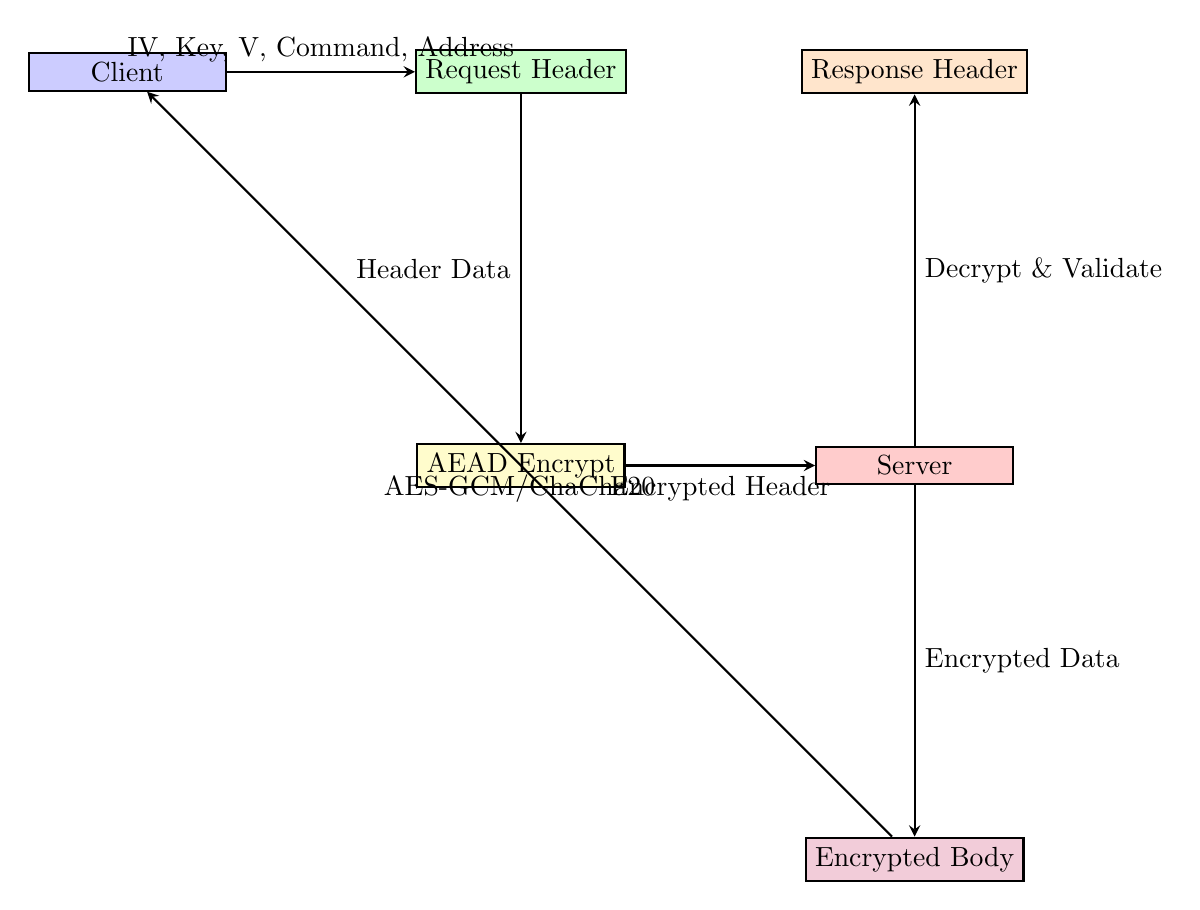
\begin{tikzpicture}[node distance=5cm,>=stealth,thick]
        \node (client) [draw, rectangle, fill=blue!20, minimum width=2.5cm] {Client};
        \node (req) [draw, rectangle, right of=client, fill=green!20, minimum width=2cm] {Request Header};
        \node (enc) [draw, rectangle, below of=req, fill=yellow!20, minimum width=2cm] {AEAD Encrypt};
        \node (server) [draw, rectangle, right of=enc, fill=red!20, minimum width=2.5cm] {Server};
        \node (resp) [draw, rectangle, above of=server, fill=orange!20, minimum width=2cm] {Response Header};
        \node (body) [draw, rectangle, below of=server, fill=purple!20, minimum width=2cm] {Encrypted Body};
        
        \draw[->] (client) -- node[above] {IV, Key, V, Command, Address} (req);
        \draw[->] (req) -- node[left] {Header Data} (enc);
        \draw[->] (enc) -- node[below] {Encrypted Header} (server);
        \draw[->] (server) -- node[right] {Decrypt \& Validate} (resp);
        \draw[->] (server) -- node[right] {Encrypted Data} (body);
        \draw[->] (body) -- node[below] {AES-GCM/ChaCha20} (client);
    \end{tikzpicture}
    \caption{VMESS Protocol Handshake and Data Flow}
\end{figure}

\subsection{VMESS Time-Based Authentication}

VMESS requires accurate system time for authentication. The server validates:

\[
|\text{ServerTime} - \text{ClientTime}| < 120 \text{ seconds}
\]

The authentication uses HMAC-SHA256:

\[
\text{Auth} = \text{HMAC-SHA256}(K_{\text{cmd}}, \text{Header} || \text{Timestamp})
\]

\subsection{VMESS Chunk Stream}

VMESS supports chunked streaming with size masking:

\[
\text{EncryptedSize} = \text{Size} \oplus \text{SHAKE-128}(\text{IV})[0:2]
\]

\begin{verbatim}
// From Xray-core: proxy/vmess/encoding/auth.go
type ShakeSizeParser struct {
    shake  sha3.ShakeHash
    buffer [2]byte
}

func (s *ShakeSizeParser) Encode(size uint16, b []byte) []byte {
    mask := s.next()  // Get 2 bytes from SHAKE-128 stream
    binary.BigEndian.PutUint16(b, mask^size)
    return b[:2]
}
\end{verbatim}

\section{VLESS Protocol}

VLESS (Versatile Lightweight Encrypted Stream) is a simplified, stateless protocol designed for better performance and flexibility. It supports advanced features like XTLS (eXtended TLS) for zero-copy optimization.

\subsection{Protocol Overview}

VLESS is simpler than VMESS:
\begin{itemize}
    \item \textbf{UUID}: 16-byte identifier (required, no alterId)
    \item \textbf{Encryption}: Optional (default: "none")
    \item \textbf{Flow}: Optional flow control (e.g., "xtls-rprx-vision")
    \item \textbf{No Time Sync}: Unlike VMESS, VLESS doesn't require time synchronization
\end{itemize}

\subsection{VLESS Request Header}

The VLESS request header is much simpler than VMESS:

\begin{verbatim}
// From Xray-core: proxy/vless/encoding/encoding.go
type RequestHeader struct {
    Version byte              // Always 0
    UUID    [16]byte          // User UUID
    Addons  *Addons           // Flow and other addons
    Command RequestCommand    // TCP, UDP, Mux, Rvs
    Address net.Address       // Destination
    Port    net.Port          // Destination port
}
\end{verbatim}

\subsubsection{Header Encoding}

\begin{verbatim}
// From Xray-core: proxy/vless/encoding/encoding.go
func EncodeRequestHeader(writer io.Writer, request *protocol.RequestHeader, requestAddons *Addons) error {
    buffer := buf.StackNew()
    
    buffer.WriteByte(request.Version)  // Version = 0
    buffer.Write(request.User.Account.(*vless.MemoryAccount).ID.Bytes())  // 16 bytes UUID
    
    // Encode addons (flow, etc.)
    EncodeHeaderAddons(&buffer, requestAddons)
    
    buffer.WriteByte(byte(request.Command))  // Command
    
    // Address and port (if not Mux/Rvs)
    if request.Command != protocol.RequestCommandMux && 
       request.Command != protocol.RequestCommandRvs {
        addrParser.WriteAddressPort(&buffer, request.Address, request.Port)
    }
    
    writer.Write(buffer.Bytes())
    return nil
}
\end{verbatim}

\subsection{VLESS Encryption (Optional)}

VLESS supports optional encryption using X25519 and ML-KEM-768:

\subsubsection{X25519 Key Exchange}

\[
\text{Client}: a \in_R [0, 2^{256}), A = aG
\]
\[
\text{Server}: B \text{ (public key)}
\]
\[
\text{Shared Secret}: S = aB = abG
\]
\[
\text{Derived Key}: K = \text{BLAKE3}(S)
\]

\subsubsection{ML-KEM-768 Post-Quantum Key Exchange}

\[
\text{Server}: (sk, pk) = \text{ML-KEM-768.KeyGen}()
\]
\[
\text{Client}: (K, ct) = \text{ML-KEM-768.Encaps}(pk)
\]
\[
\text{Server}: K' = \text{ML-KEM-768.Decaps}(sk, ct)
\]

\begin{verbatim}
// From Xray-core: proxy/vless/encryption/client.go
func (i *ClientInstance) Handshake(conn net.Conn) (*CommonConn, error) {
    // Generate IV
    iv := make([]byte, 16)
    rand.Read(iv)
    
    // Perform key exchange for each relay
    for j, k := range i.NfsPKeys {
        if k, ok := k.(*ecdh.PublicKey); ok {
            // X25519 key exchange
            privateKey, _ := ecdh.X25519().GenerateKey(rand.Reader)
            nfsKey, err := privateKey.ECDH(k)
            // ...
        } else if k, ok := k.(*mlkem.EncapsulationKey768); ok {
            // ML-KEM-768 key exchange
            nfsKey, ciphertext := k.Encapsulate()
            // ...
        }
    }
    
    // Create AEAD from derived keys
    nfsAEAD := NewAEAD(iv, nfsKey, useAES)
    // ...
}
\end{verbatim}

\subsection{VLESS XTLS Flow}

XTLS (eXtended TLS) is a zero-copy optimization that allows direct splicing of TLS connections:

\subsubsection{xtls-rprx-vision Flow}

The "xtls-rprx-vision" flow enables:
\begin{itemize}
    \item \textbf{Zero-Copy}: Direct memory copy without encryption/decryption
    \item \textbf{TLS 1.3 Only}: Requires TLS 1.3 for security
    \item \textbf{Traffic Obfuscation}: Makes traffic patterns less distinguishable
\end{itemize}

\begin{verbatim}
// From Xray-core: proxy/vless/outbound/outbound.go
if requestAddons.Flow == vless.XRV {
    // XTLS Vision flow
    ob.CanSpliceCopy = 2  // Enable zero-copy
    
    // Access TLS connection's internal buffers
    if tlsConn, ok := iConn.(*tls.Conn); ok {
        if tlsConn.ConnectionState().Version != gotls.VersionTLS13 {
            return errors.New("XTLS requires TLS 1.3")
        }
        // Direct access to TLS input buffer for zero-copy
        input = (*bytes.Reader)(unsafe.Pointer(p + i.Offset))
        rawInput = (*bytes.Buffer)(unsafe.Pointer(p + r.Offset))
    }
}
\end{verbatim}

\begin{figure}[h]
    \centering
    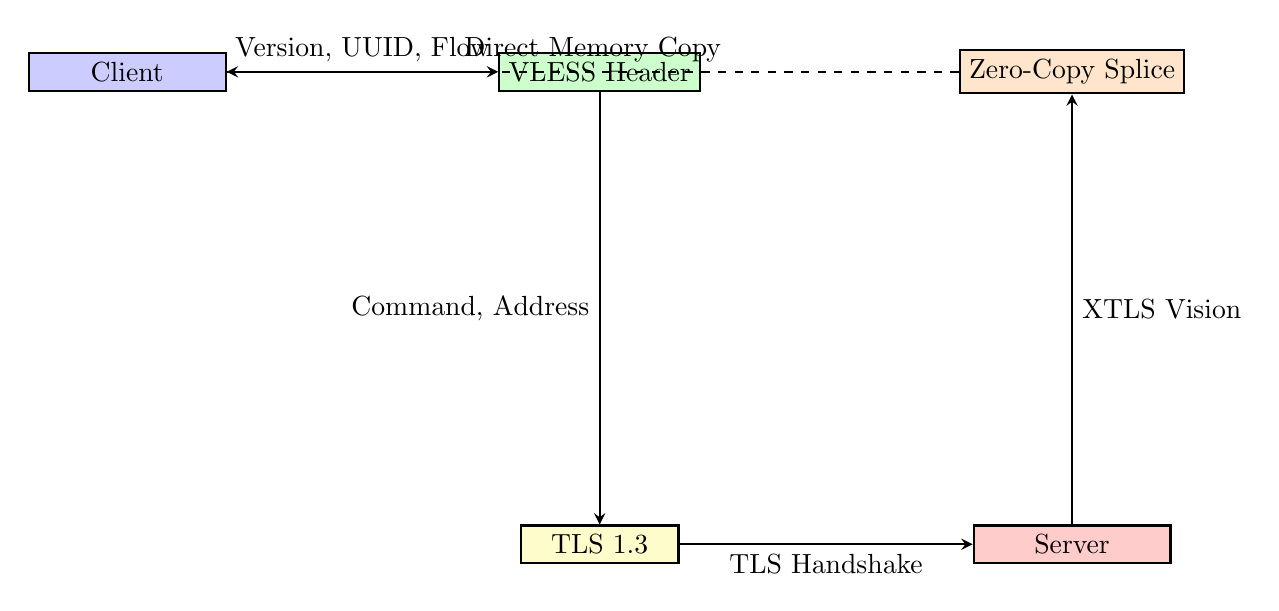
\begin{tikzpicture}[node distance=6cm,>=stealth,thick]
        \node (client) [draw, rectangle, fill=blue!20, minimum width=2.5cm] {Client};
        \node (header) [draw, rectangle, right of=client, fill=green!20, minimum width=2cm] {VLESS Header};
        \node (tls) [draw, rectangle, below of=header, fill=yellow!20, minimum width=2cm] {TLS 1.3};
        \node (server) [draw, rectangle, right of=tls, fill=red!20, minimum width=2.5cm] {Server};
        \node (splice) [draw, rectangle, above of=server, fill=orange!20, minimum width=2cm] {Zero-Copy Splice};
        
        \draw[->] (client) -- node[above] {Version, UUID, Flow} (header);
        \draw[->] (header) -- node[left] {Command, Address} (tls);
        \draw[->] (tls) -- node[below] {TLS Handshake} (server);
        \draw[->] (server) -- node[right] {XTLS Vision} (splice);
        \draw[->, dashed] (splice) -- node[above] {Direct Memory Copy} (client);
    \end{tikzpicture}
    \caption{VLESS Protocol with XTLS Vision Flow}
\end{figure}

\subsection{VLESS Response Header}

The VLESS response header is minimal:

\begin{verbatim}
type ResponseHeader struct {
    Version byte    // Echo request version
    Addons  *Addons // Response addons
}
\end{verbatim}

\section{Trojan Protocol}

Trojan is a simple, stateless protocol that mimics HTTPS traffic. It uses password-based authentication and relies on TLS for encryption.

\subsection{Protocol Overview}

Trojan is designed to be indistinguishable from HTTPS:
\begin{itemize}
    \item \textbf{Password}: SHA-224 hash of user password (56 bytes)
    \item \textbf{TLS Required}: All traffic must be wrapped in TLS
    \item \textbf{Simple Header}: Minimal protocol overhead
    \item \textbf{No Encryption}: Trojan itself doesn't encrypt; relies on TLS
\end{itemize}

\subsection{Trojan Request Header}

The Trojan request header is extremely simple:

\begin{verbatim}
// From Xray-core: proxy/trojan/protocol.go
type RequestHeader struct {
    Password [56]byte    // SHA-224 hash of password
    CRLF     [2]byte     // \r\n
    Command  byte        // 1 = TCP, 3 = UDP
    Address  net.Address // Destination address
    Port     net.Port    // Destination port
    CRLF     [2]byte     // \r\n
}
\end{verbatim}

\subsubsection{Header Encoding}

\begin{verbatim}
// From Xray-core: proxy/trojan/protocol.go
func (c *ConnWriter) writeHeader() error {
    buffer := buf.StackNew()
    
    // Write password hash (56 bytes)
    buffer.Write(c.Account.Key)  // SHA-224 hash
    
    // Write CRLF
    buffer.Write([]byte{'\r', '\n'})
    
    // Write command (1 = TCP, 3 = UDP)
    command := commandTCP
    if c.Target.Network == net.Network_UDP {
        command = commandUDP
    }
    buffer.WriteByte(command)
    
    // Write address and port
    addrParser.WriteAddressPort(&buffer, c.Target.Address, c.Target.Port)
    
    // Write CRLF
    buffer.Write([]byte{'\r', '\n'})
    
    c.Writer.Write(buffer.Bytes())
    c.headerSent = true
    return nil
}
\end{verbatim}

\subsection{Trojan Password Authentication}

Trojan uses SHA-224 hash of the password:

\[
K = \text{SHA-224}(\text{Password})
\]

The server validates the password hash:

\begin{verbatim}
// From Xray-core: proxy/trojan/validator.go
type Validator struct {
    email sync.Map
    users sync.Map  // Key: hex string of SHA-224 hash
}

func (v *Validator) Get(hash string) *protocol.MemoryUser {
    u, _ := v.users.Load(hash)
    if u != nil {
        return u.(*protocol.MemoryUser)
    }
    return nil
}
\end{verbatim}

\subsection{Trojan UDP Protocol}

For UDP packets, Trojan uses a different format:

\begin{verbatim}
// UDP Packet Format:
// [Address][Port][Length (2 bytes)][CRLF][Payload]
func (w *PacketWriter) writePacket(payload []byte, dest net.Destination) (int, error) {
    buffer := buf.StackNew()
    
    // Write address and port
    addrParser.WriteAddressPort(&buffer, dest.Address, dest.Port)
    
    // Write payload length (2 bytes, big-endian)
    lengthBuf := [2]byte{}
    binary.BigEndian.PutUint16(lengthBuf[:], uint16(len(payload)))
    buffer.Write(lengthBuf[:])
    
    // Write CRLF
    buffer.Write([]byte{'\r', '\n'})
    
    // Write payload
    buffer.Write(payload)
    
    w.Write(buffer.Bytes())
    return len(payload), nil
}
\end{verbatim}

\begin{figure}[h]
    \centering
    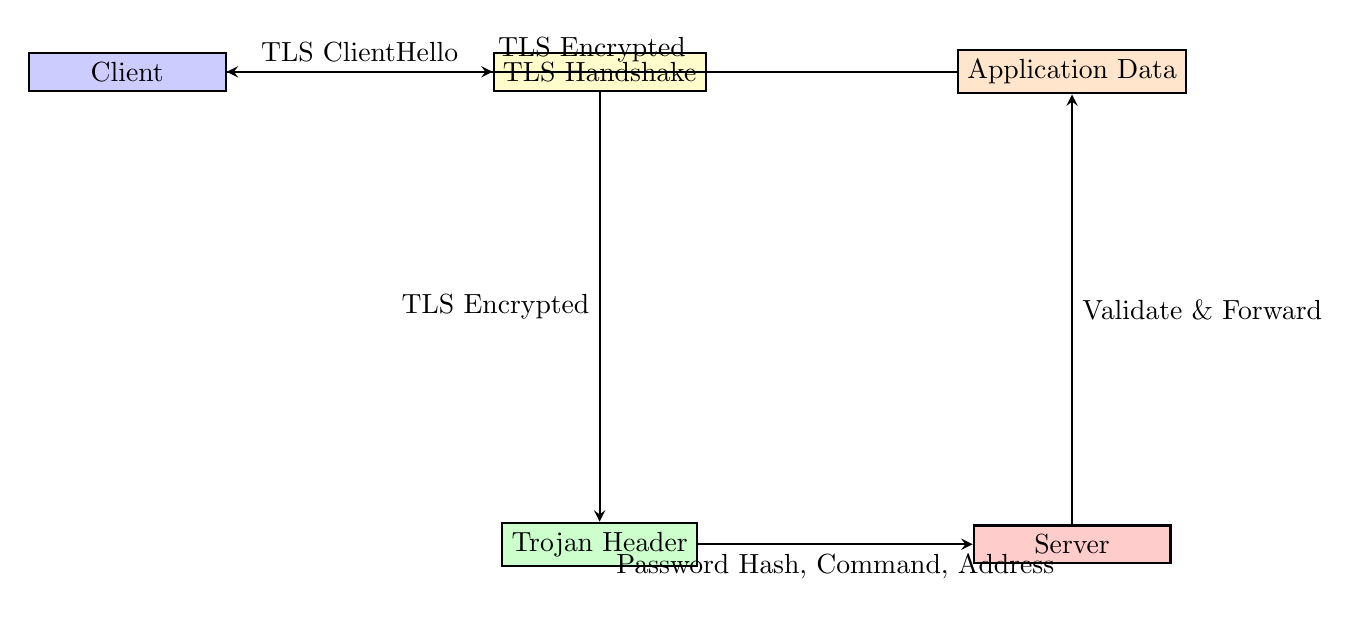
\begin{tikzpicture}[node distance=6cm,>=stealth,thick]
        \node (client) [draw, rectangle, fill=blue!20, minimum width=2.5cm] {Client};
        \node (tls) [draw, rectangle, right of=client, fill=yellow!20, minimum width=2cm] {TLS Handshake};
        \node (header) [draw, rectangle, below of=tls, fill=green!20, minimum width=2cm] {Trojan Header};
        \node (server) [draw, rectangle, right of=header, fill=red!20, minimum width=2.5cm] {Server};
        \node (data) [draw, rectangle, above of=server, fill=orange!20, minimum width=2cm] {Application Data};
        
        \draw[->] (client) -- node[above] {TLS ClientHello} (tls);
        \draw[->] (tls) -- node[left] {TLS Encrypted} (header);
        \draw[->] (header) -- node[below] {Password Hash, Command, Address} (server);
        \draw[->] (server) -- node[right] {Validate \& Forward} (data);
        \draw[->] (data) -- node[above] {TLS Encrypted} (client);
    \end{tikzpicture}
    \caption{Trojan Protocol Flow (TLS-Wrapped)}
\end{figure}

\section{Protocol Comparison}

\subsection{Feature Comparison}

\begin{table}[h]
\centering
\begin{tabular}{|l|c|c|c|}
\hline
\textbf{Feature} & \textbf{VMESS} & \textbf{VLESS} & \textbf{Trojan} \\
\hline
Authentication & UUID + Time & UUID & Password Hash \\
Time Sync Required & Yes (±120s) & No & No \\
Encryption & Multiple (AES-GCM, ChaCha20) & Optional & TLS Only \\
Header Size & ~50-100 bytes & ~20-30 bytes & ~70 bytes \\
Stateful & Yes & No & No \\
Zero-Copy (XTLS) & No & Yes (Vision) & No \\
Post-Quantum & No & Yes (ML-KEM-768) & No \\
Complexity & High & Medium & Low \\
\hline
\end{tabular}
\caption{Protocol Feature Comparison}
\end{table}

\subsection{Performance Characteristics}

\subsubsection{VMESS}
\begin{itemize}
    \item \textbf{Overhead}: ~50-100 bytes per connection (header)
    \item \textbf{Encryption}: AES-128-GCM or ChaCha20-Poly1305
    \item \textbf{Latency}: Higher due to time-based authentication
    \item \textbf{Throughput}: Good, but not optimal
\end{itemize}

\subsubsection{VLESS}
\begin{itemize}
    \item \textbf{Overhead}: ~20-30 bytes per connection (minimal header)
    \item \textbf{Encryption}: Optional, can use TLS or custom encryption
    \item \textbf{Latency}: Lower (no time sync requirement)
    \item \textbf{Throughput}: Excellent with XTLS Vision (zero-copy)
\end{itemize}

\subsubsection{Trojan}
\begin{itemize}
    \item \textbf{Overhead}: ~70 bytes per connection (header + TLS)
    \item \textbf{Encryption}: TLS (typically TLS 1.3)
    \item \textbf{Latency}: Low (simple protocol)
    \item \textbf{Throughput}: Good (TLS hardware acceleration)
\end{itemize}

\section{Security Analysis}

\subsection{VMESS Security}

\begin{itemize}
    \item \textbf{Authentication}: Strong (UUID + time-based)
    \item \textbf{Encryption}: Strong (AES-128-GCM, ChaCha20-Poly1305)
    \item \textbf{Forward Secrecy}: Limited (session keys derived from UUID)
    \item \textbf{Traffic Analysis}: Moderate resistance (padding, chunk masking)
\end{itemize}

\subsection{VLESS Security}

\begin{itemize}
    \item \textbf{Authentication}: Moderate (UUID only)
    \item \textbf{Encryption}: Strong (when enabled, supports post-quantum)
    \item \textbf{Forward Secrecy}: Excellent (X25519 + ML-KEM-768)
    \item \textbf{Traffic Analysis}: Good resistance (XTLS Vision obfuscation)
\end{itemize}

\subsection{Trojan Security}

\begin{itemize}
    \item \textbf{Authentication}: Weak (password hash only)
    \item \textbf{Encryption}: Strong (TLS, typically TLS 1.3)
    \item \textbf{Forward Secrecy}: Excellent (TLS 1.3 provides PFS)
    \item \textbf{Traffic Analysis}: Excellent (indistinguishable from HTTPS)
\end{itemize}

\section{Implementation Details}

\subsection{VMESS Session Management}

VMESS maintains session state for encryption:

\begin{verbatim}
// From Xray-core: proxy/vmess/encoding/client.go
type ClientSession struct {
    requestBodyKey  [16]byte
    requestBodyIV   [16]byte
    responseBodyKey [16]byte
    responseBodyIV  [16]byte
    responseReader  io.Reader
    responseHeader  byte
}
\end{verbatim}

\subsection{VLESS Connection Reuse}

VLESS supports connection pre-connection for reduced latency:

\begin{verbatim}
// From Xray-core: proxy/vless/outbound/outbound.go
if h.testpre > 0 {
    // Pre-connect connections in background
    h.preConns = make(chan *ConnExpire)
    for range h.testpre {
        go func() {
            conn, _ := dialer.Dial(ctx, rec.Destination)
            h.preConns <- &ConnExpire{Conn: conn, Expire: time.Now().Add(2 * time.Minute)}
        }()
    }
}
\end{verbatim}

\subsection{Trojan Validator}

Trojan uses a hash map for fast password lookup:

\begin{verbatim}
// From Xray-core: proxy/trojan/validator.go
type Validator struct {
    email sync.Map  // Email -> User mapping
    users sync.Map  // SHA-224 hash -> User mapping
}

func (v *Validator) Add(u *protocol.MemoryUser) error {
    key := hexString(u.Account.(*MemoryAccount).Key)  // SHA-224 hash as hex
    v.users.Store(key, u)
    return nil
}
\end{verbatim}

\section{Summary}

This chapter covered the three major proxy protocols:

\begin{itemize}
    \item \textbf{VMESS}: Feature-rich protocol with time-based authentication, multiple encryption methods, and chunk masking
    \item \textbf{VLESS}: Simplified protocol with optional encryption, XTLS support for zero-copy, and post-quantum key exchange
    \item \textbf{Trojan}: Simple protocol that mimics HTTPS, uses password authentication, and relies on TLS for encryption
\end{itemize}

Each protocol has its strengths:
\begin{itemize}
    \item \textbf{VMESS}: Best for compatibility and feature support
    \item \textbf{VLESS}: Best for performance and modern features
    \item \textbf{Trojan}: Best for traffic obfuscation and simplicity
\end{itemize}

Understanding these protocols is essential for:
\begin{itemize}
    \item Choosing the right protocol for your use case
    \item Debugging connection issues
    \item Optimizing performance
    \item Implementing protocol extensions
\end{itemize}


\chapter{Appendix: Useful Commands}

\begin{itemize}
    \item Run control plane: \texttt{smart-relay serve --listen 0.0.0.0:8080}
    \item Ask AI for plan: \texttt{smart-relay propose --goal "streaming EU first"}
    \item Validate config: \texttt{smart-relay validate}
    \item Set Ollama host: \texttt{set OLLAMA\_HOST=http://localhost:11434}
\end{itemize}



\end{document}

